% Options for packages loaded elsewhere
% Options for packages loaded elsewhere
\PassOptionsToPackage{unicode}{hyperref}
\PassOptionsToPackage{hyphens}{url}
\PassOptionsToPackage{dvipsnames,svgnames,x11names}{xcolor}
%
\documentclass[
  letterpaper,
  DIV=11,
  numbers=noendperiod]{scrreprt}
\usepackage{xcolor}
\usepackage{amsmath,amssymb}
\setcounter{secnumdepth}{5}
\usepackage{iftex}
\ifPDFTeX
  \usepackage[T1]{fontenc}
  \usepackage[utf8]{inputenc}
  \usepackage{textcomp} % provide euro and other symbols
\else % if luatex or xetex
  \usepackage{unicode-math} % this also loads fontspec
  \defaultfontfeatures{Scale=MatchLowercase}
  \defaultfontfeatures[\rmfamily]{Ligatures=TeX,Scale=1}
\fi
\usepackage{lmodern}
\ifPDFTeX\else
  % xetex/luatex font selection
\fi
% Use upquote if available, for straight quotes in verbatim environments
\IfFileExists{upquote.sty}{\usepackage{upquote}}{}
\IfFileExists{microtype.sty}{% use microtype if available
  \usepackage[]{microtype}
  \UseMicrotypeSet[protrusion]{basicmath} % disable protrusion for tt fonts
}{}
\makeatletter
\@ifundefined{KOMAClassName}{% if non-KOMA class
  \IfFileExists{parskip.sty}{%
    \usepackage{parskip}
  }{% else
    \setlength{\parindent}{0pt}
    \setlength{\parskip}{6pt plus 2pt minus 1pt}}
}{% if KOMA class
  \KOMAoptions{parskip=half}}
\makeatother
% Make \paragraph and \subparagraph free-standing
\makeatletter
\ifx\paragraph\undefined\else
  \let\oldparagraph\paragraph
  \renewcommand{\paragraph}{
    \@ifstar
      \xxxParagraphStar
      \xxxParagraphNoStar
  }
  \newcommand{\xxxParagraphStar}[1]{\oldparagraph*{#1}\mbox{}}
  \newcommand{\xxxParagraphNoStar}[1]{\oldparagraph{#1}\mbox{}}
\fi
\ifx\subparagraph\undefined\else
  \let\oldsubparagraph\subparagraph
  \renewcommand{\subparagraph}{
    \@ifstar
      \xxxSubParagraphStar
      \xxxSubParagraphNoStar
  }
  \newcommand{\xxxSubParagraphStar}[1]{\oldsubparagraph*{#1}\mbox{}}
  \newcommand{\xxxSubParagraphNoStar}[1]{\oldsubparagraph{#1}\mbox{}}
\fi
\makeatother

\usepackage{color}
\usepackage{fancyvrb}
\newcommand{\VerbBar}{|}
\newcommand{\VERB}{\Verb[commandchars=\\\{\}]}
\DefineVerbatimEnvironment{Highlighting}{Verbatim}{commandchars=\\\{\}}
% Add ',fontsize=\small' for more characters per line
\usepackage{framed}
\definecolor{shadecolor}{RGB}{241,243,245}
\newenvironment{Shaded}{\begin{snugshade}}{\end{snugshade}}
\newcommand{\AlertTok}[1]{\textcolor[rgb]{0.68,0.00,0.00}{#1}}
\newcommand{\AnnotationTok}[1]{\textcolor[rgb]{0.37,0.37,0.37}{#1}}
\newcommand{\AttributeTok}[1]{\textcolor[rgb]{0.40,0.45,0.13}{#1}}
\newcommand{\BaseNTok}[1]{\textcolor[rgb]{0.68,0.00,0.00}{#1}}
\newcommand{\BuiltInTok}[1]{\textcolor[rgb]{0.00,0.23,0.31}{#1}}
\newcommand{\CharTok}[1]{\textcolor[rgb]{0.13,0.47,0.30}{#1}}
\newcommand{\CommentTok}[1]{\textcolor[rgb]{0.37,0.37,0.37}{#1}}
\newcommand{\CommentVarTok}[1]{\textcolor[rgb]{0.37,0.37,0.37}{\textit{#1}}}
\newcommand{\ConstantTok}[1]{\textcolor[rgb]{0.56,0.35,0.01}{#1}}
\newcommand{\ControlFlowTok}[1]{\textcolor[rgb]{0.00,0.23,0.31}{\textbf{#1}}}
\newcommand{\DataTypeTok}[1]{\textcolor[rgb]{0.68,0.00,0.00}{#1}}
\newcommand{\DecValTok}[1]{\textcolor[rgb]{0.68,0.00,0.00}{#1}}
\newcommand{\DocumentationTok}[1]{\textcolor[rgb]{0.37,0.37,0.37}{\textit{#1}}}
\newcommand{\ErrorTok}[1]{\textcolor[rgb]{0.68,0.00,0.00}{#1}}
\newcommand{\ExtensionTok}[1]{\textcolor[rgb]{0.00,0.23,0.31}{#1}}
\newcommand{\FloatTok}[1]{\textcolor[rgb]{0.68,0.00,0.00}{#1}}
\newcommand{\FunctionTok}[1]{\textcolor[rgb]{0.28,0.35,0.67}{#1}}
\newcommand{\ImportTok}[1]{\textcolor[rgb]{0.00,0.46,0.62}{#1}}
\newcommand{\InformationTok}[1]{\textcolor[rgb]{0.37,0.37,0.37}{#1}}
\newcommand{\KeywordTok}[1]{\textcolor[rgb]{0.00,0.23,0.31}{\textbf{#1}}}
\newcommand{\NormalTok}[1]{\textcolor[rgb]{0.00,0.23,0.31}{#1}}
\newcommand{\OperatorTok}[1]{\textcolor[rgb]{0.37,0.37,0.37}{#1}}
\newcommand{\OtherTok}[1]{\textcolor[rgb]{0.00,0.23,0.31}{#1}}
\newcommand{\PreprocessorTok}[1]{\textcolor[rgb]{0.68,0.00,0.00}{#1}}
\newcommand{\RegionMarkerTok}[1]{\textcolor[rgb]{0.00,0.23,0.31}{#1}}
\newcommand{\SpecialCharTok}[1]{\textcolor[rgb]{0.37,0.37,0.37}{#1}}
\newcommand{\SpecialStringTok}[1]{\textcolor[rgb]{0.13,0.47,0.30}{#1}}
\newcommand{\StringTok}[1]{\textcolor[rgb]{0.13,0.47,0.30}{#1}}
\newcommand{\VariableTok}[1]{\textcolor[rgb]{0.07,0.07,0.07}{#1}}
\newcommand{\VerbatimStringTok}[1]{\textcolor[rgb]{0.13,0.47,0.30}{#1}}
\newcommand{\WarningTok}[1]{\textcolor[rgb]{0.37,0.37,0.37}{\textit{#1}}}

\usepackage{longtable,booktabs,array}
\usepackage{calc} % for calculating minipage widths
% Correct order of tables after \paragraph or \subparagraph
\usepackage{etoolbox}
\makeatletter
\patchcmd\longtable{\par}{\if@noskipsec\mbox{}\fi\par}{}{}
\makeatother
% Allow footnotes in longtable head/foot
\IfFileExists{footnotehyper.sty}{\usepackage{footnotehyper}}{\usepackage{footnote}}
\makesavenoteenv{longtable}
\usepackage{graphicx}
\makeatletter
\newsavebox\pandoc@box
\newcommand*\pandocbounded[1]{% scales image to fit in text height/width
  \sbox\pandoc@box{#1}%
  \Gscale@div\@tempa{\textheight}{\dimexpr\ht\pandoc@box+\dp\pandoc@box\relax}%
  \Gscale@div\@tempb{\linewidth}{\wd\pandoc@box}%
  \ifdim\@tempb\p@<\@tempa\p@\let\@tempa\@tempb\fi% select the smaller of both
  \ifdim\@tempa\p@<\p@\scalebox{\@tempa}{\usebox\pandoc@box}%
  \else\usebox{\pandoc@box}%
  \fi%
}
% Set default figure placement to htbp
\def\fps@figure{htbp}
\makeatother





\setlength{\emergencystretch}{3em} % prevent overfull lines

\providecommand{\tightlist}{%
  \setlength{\itemsep}{0pt}\setlength{\parskip}{0pt}}



 


\KOMAoption{captions}{tableheading}
\makeatletter
\@ifpackageloaded{tcolorbox}{}{\usepackage[skins,breakable]{tcolorbox}}
\@ifpackageloaded{fontawesome5}{}{\usepackage{fontawesome5}}
\definecolor{quarto-callout-color}{HTML}{909090}
\definecolor{quarto-callout-note-color}{HTML}{0758E5}
\definecolor{quarto-callout-important-color}{HTML}{CC1914}
\definecolor{quarto-callout-warning-color}{HTML}{EB9113}
\definecolor{quarto-callout-tip-color}{HTML}{00A047}
\definecolor{quarto-callout-caution-color}{HTML}{FC5300}
\definecolor{quarto-callout-color-frame}{HTML}{acacac}
\definecolor{quarto-callout-note-color-frame}{HTML}{4582ec}
\definecolor{quarto-callout-important-color-frame}{HTML}{d9534f}
\definecolor{quarto-callout-warning-color-frame}{HTML}{f0ad4e}
\definecolor{quarto-callout-tip-color-frame}{HTML}{02b875}
\definecolor{quarto-callout-caution-color-frame}{HTML}{fd7e14}
\makeatother
\makeatletter
\@ifpackageloaded{bookmark}{}{\usepackage{bookmark}}
\makeatother
\makeatletter
\@ifpackageloaded{caption}{}{\usepackage{caption}}
\AtBeginDocument{%
\ifdefined\contentsname
  \renewcommand*\contentsname{Table of contents}
\else
  \newcommand\contentsname{Table of contents}
\fi
\ifdefined\listfigurename
  \renewcommand*\listfigurename{List of Figures}
\else
  \newcommand\listfigurename{List of Figures}
\fi
\ifdefined\listtablename
  \renewcommand*\listtablename{List of Tables}
\else
  \newcommand\listtablename{List of Tables}
\fi
\ifdefined\figurename
  \renewcommand*\figurename{Figure}
\else
  \newcommand\figurename{Figure}
\fi
\ifdefined\tablename
  \renewcommand*\tablename{Table}
\else
  \newcommand\tablename{Table}
\fi
}
\@ifpackageloaded{float}{}{\usepackage{float}}
\floatstyle{ruled}
\@ifundefined{c@chapter}{\newfloat{codelisting}{h}{lop}}{\newfloat{codelisting}{h}{lop}[chapter]}
\floatname{codelisting}{Listing}
\newcommand*\listoflistings{\listof{codelisting}{List of Listings}}
\usepackage{amsthm}
\theoremstyle{definition}
\newtheorem{definition}{Definition}[chapter]
\theoremstyle{definition}
\newtheorem{example}{Example}[chapter]
\theoremstyle{remark}
\AtBeginDocument{\renewcommand*{\proofname}{Proof}}
\newtheorem*{remark}{Remark}
\newtheorem*{solution}{Solution}
\newtheorem{refremark}{Remark}[chapter]
\newtheorem{refsolution}{Solution}[chapter]
\makeatother
\makeatletter
\makeatother
\makeatletter
\@ifpackageloaded{caption}{}{\usepackage{caption}}
\@ifpackageloaded{subcaption}{}{\usepackage{subcaption}}
\makeatother
\usepackage{bookmark}
\IfFileExists{xurl.sty}{\usepackage{xurl}}{} % add URL line breaks if available
\urlstyle{same}
\hypersetup{
  pdftitle={MAS2901: Statistical Inference},
  pdfauthor={Matthew Fisher},
  colorlinks=true,
  linkcolor={blue},
  filecolor={Maroon},
  citecolor={Blue},
  urlcolor={Blue},
  pdfcreator={LaTeX via pandoc}}


\title{MAS2901: Statistical Inference}
\author{Matthew Fisher}
\date{}
\begin{document}
\maketitle

\renewcommand*\contentsname{Table of contents}
{
\hypersetup{linkcolor=}
\setcounter{tocdepth}{2}
\tableofcontents
}

\bookmarksetup{startatroot}

\chapter*{Preface}\label{preface}
\addcontentsline{toc}{chapter}{Preface}

\markboth{Preface}{Preface}

Welcome to the online notes for \textbf{MAS2901 --- Statistical
Inference}.

This 10-credit module at Newcastle University introduces the two main
approaches to \emph{statistical inference}:

\begin{itemize}
\tightlist
\item
  \textbf{Frequentist inference}
\item
  \textbf{Bayesian inference}
\end{itemize}

\section*{What is Statistical
Inference?}\label{what-is-statistical-inference}
\addcontentsline{toc}{section}{What is Statistical Inference?}

\markright{What is Statistical Inference?}

Statistical inference is the process of using data from a \emph{sample}
to learn about a \emph{population}. Sometimes the population is concrete
(e.g.~``all people in the country today''). In other situations we want
to generalise beyond those we sampled to a broader \emph{target
population} (sometimes called a \emph{superpopulation}), such as
``future patients with similar characteristics''. Clear definitions and
sensible assumptions are essential for valid conclusions.

There are two main types of statistical inference:

\begin{itemize}
\tightlist
\item
  \textbf{Frequentist inference.} Parameters are treated as
  \textbf{fixed but unknown}. Probability statements are about
  \emph{data we might observe} under repeated sampling from the same
  model.
\item
  \textbf{Bayesian inference.} Parameters are treated as \textbf{random}
  with a \emph{prior distribution}. Probability statements are about the
  \emph{parameter given the data} via the posterior distribution.
\end{itemize}

The examples below are only to build intuition about the core difference
between frequentist and Bayesian inference. Don't worry about the
details---we'll cover them carefully later in the course.

\begin{example}[A comparison of Frequentist vs Bayesian
inference]\protect\hypertarget{exm-proportion-freq-bayes}{}\label{exm-proportion-freq-bayes}

A survey asks \(n=20\) students if they prefer study space \(A\) or
\(B\).

Suppose \(x=12\) prefer \(A\). Compare a frequentist and a Bayesian
estimate of the long-run proportion \(p\) who would choose \(A\).

\end{example}

\begin{tcolorbox}[enhanced jigsaw, left=2mm, titlerule=0mm, bottomrule=.15mm, colframe=quarto-callout-tip-color-frame, arc=.35mm, colback=white, breakable, title=\textcolor{quarto-callout-tip-color}{\faLightbulb}\hspace{0.5em}{Solution}, colbacktitle=quarto-callout-tip-color!10!white, opacitybacktitle=0.6, opacityback=0, toprule=.15mm, leftrule=.75mm, coltitle=black, toptitle=1mm, rightrule=.15mm, bottomtitle=1mm]

\textbf{Frequentist.} The natural estimator is the sample proportion

\[
\hat p=\frac{x}{n}=\frac{12}{20}=0.60.
\]

\textbf{Bayesian (with a uniform prior).} Take a \(\mathrm{Beta}(1,1)\)
prior for \(p\). The posterior is

\[
p \mid x \sim \mathrm{Beta}(1+x,\,1+n-x)=\mathrm{Beta}(13,9),
\]

whose mean is

\[
\mathbb{E}[p\mid x]=\frac{13}{13+9}=\frac{13}{22}\approx 0.591.
\]

\textbf{Interpretation.} The frequentist estimate \(\hat p\) is a
function of the data and treats \(p\) as fixed.\\
The Bayesian estimate is an expectation \emph{of \(p\) itself} under the
posterior distribution.

\end{tcolorbox}

\begin{center}\rule{0.5\linewidth}{0.5pt}\end{center}

\begin{example}[Interpreting probability
statements]\protect\hypertarget{exm-interpretations}{}\label{exm-interpretations}

Decide whether each statement is \emph{frequentist} or \emph{Bayesian}
in spirit.

\begin{enumerate}
\def\labelenumi{\arabic{enumi}.}
\tightlist
\item
  ``If we repeated the survey many times, the method we use would
  produce intervals that capture \(p\) about 95\% of the time.''\\
\item
  ``Given the data from this survey and our prior, there is a 95\%
  probability that \(p\) lies between 0.45 and 0.75.''
\end{enumerate}

\end{example}

\begin{tcolorbox}[enhanced jigsaw, left=2mm, titlerule=0mm, bottomrule=.15mm, colframe=quarto-callout-tip-color-frame, arc=.35mm, colback=white, breakable, title=\textcolor{quarto-callout-tip-color}{\faLightbulb}\hspace{0.5em}{Solution}, colbacktitle=quarto-callout-tip-color!10!white, opacitybacktitle=0.6, opacityback=0, toprule=.15mm, leftrule=.75mm, coltitle=black, toptitle=1mm, rightrule=.15mm, bottomtitle=1mm]

\begin{enumerate}
\def\labelenumi{\arabic{enumi}.}
\tightlist
\item
  \textbf{Frequentist.} This describes \emph{long-run coverage} of a
  procedure over repeated samples with \(p\) fixed.\\
\item
  \textbf{Bayesian.} This is a probability statement \emph{about \(p\)
  given the observed data} (a credible interval).
\end{enumerate}

\end{tcolorbox}

\begin{center}\rule{0.5\linewidth}{0.5pt}\end{center}

\section*{Structure of the Course}\label{structure-of-the-course}
\addcontentsline{toc}{section}{Structure of the Course}

\markright{Structure of the Course}

The notes are structured as follows:

\begin{itemize}
\item
  Part 1: Preliminaries

  \begin{itemize}
  \tightlist
  \item
    Probability Theory\\
  \item
    What is Statistical Inference? (introduces \textbf{statistical
    models})\\
  \item
    Types of Inference\\
  \end{itemize}
\item
  Part 2: Point Estimation

  \begin{itemize}
  \tightlist
  \item
    Estimate vs.~Estimator\\
  \item
    Central Limit Theorem\\
  \item
    Bias, Mean-Squared Error and Consistency\\
  \item
    Likelihood Function\\
  \item
    Bayesian Inference\\
  \end{itemize}
\item
  Part 3: Interval Estimation\\
\item
  Part 4: Hypothesis Testing\\
\item
  Part 5: Prediction
\item
  Extras:

  \begin{itemize}
  \tightlist
  \item
    Distribution Zoo (covers all the distributions used in the course)\\
  \item
    Revision Guide\\
  \item
    Question Bank
  \end{itemize}
\end{itemize}

\begin{center}\rule{0.5\linewidth}{0.5pt}\end{center}

\section*{Further Reading}\label{further-reading}
\addcontentsline{toc}{section}{Further Reading}

\markright{Further Reading}

\begin{itemize}
\tightlist
\item
  asdasdasds
\end{itemize}

\part{Part I --- Foundations}

\chapter{Probability Theory}\label{probability-theory}

\begin{tcolorbox}[enhanced jigsaw, left=2mm, titlerule=0mm, bottomrule=.15mm, colframe=quarto-callout-note-color-frame, arc=.35mm, colback=white, breakable, title=\textcolor{quarto-callout-note-color}{\faInfo}\hspace{0.5em}{Learning objectives}, colbacktitle=quarto-callout-note-color!10!white, opacitybacktitle=0.6, opacityback=0, toprule=.15mm, leftrule=.75mm, coltitle=black, toptitle=1mm, rightrule=.15mm, bottomtitle=1mm]

\begin{itemize}
\tightlist
\item
  Define and work with events (union, intersection, complement) and
  apply inclusion--exclusion.
\item
  Distinguish mutually exclusive, exhaustive, and independent events.
\item
  Compute conditional probabilities and apply Bayes' theorem.
\item
  Use partitions and the law of total probability.
\item
  Define random variables and their distribution functions: cdf, pmf
  (discrete), and pdf (continuous).
\item
  Compute probabilities from pmfs/pdfs/cdfs (using sums or areas) and
  check normalisation.
\item
  Use distribution notation \(f(x)\) with parameters \(\theta\);
  recognise \(f(x;\theta)\) (frequentist) versus \(f(x\mid \theta)\)
  (Bayesian).
\end{itemize}

\end{tcolorbox}

Before we delve into statistical inference, we briefly review key ideas
from probability theory.

\section{Probability of Events}\label{probability-of-events}

We use capital letters \(A, B,\ldots\) to denote \emph{events} (things
that may or may not occur). The complement of \(A\) is \(A^c\) (``\(A\)
does not occur'').

\begin{itemize}
\item
  \textbf{Intersection and union.} \(A\cap B\) means both \(A\)
  \emph{and} \(B\) occur. \(A\cup B\) means \(A\) \emph{or} \(B\) (or
  both) occur.
\item
  \textbf{Addition rule (inclusion--exclusion).}

  \[
  \Pr(A\cup B)=\Pr(A)+\Pr(B)-\Pr(A\cap B).
  \]
\item
  \textbf{Mutually exclusive events.} \(A\) and \(B\) are
  \emph{exclusive} if they cannot both occur; then \(\Pr(A\cap B)=0\).
\item
  \textbf{Exhaustive events.} \(A\) and \(B\) are \emph{exhaustive} if
  at least one must occur; then \(\Pr(A\cup B)=1\). (The ideas
  generalise to more than two events.)
\item
  \textbf{Independence.} Events \(A\) and \(B\) are \emph{independent}
  if

  \[
  \Pr(A\cap B)=\Pr(A)\Pr(B).
  \]
\item
  \textbf{Conditional probability.} If \(\Pr(B)>0\),

  \[
  \Pr(A\mid B)=\frac{\Pr(A\cap B)}{\Pr(B)}.
  \]
\item
  \textbf{Bayes' theorem.} If \(\Pr(B)>0\),

  \[
  \Pr(A\mid B)=\frac{\Pr(B\mid A)\Pr(A)}{\Pr(B)}.
  \]
\item
  \textbf{Partitions and the law of total probability.} Events
  \(B_1,\dots,B_n\) form a \emph{partition} if exactly one occurs
  (mutually exclusive and exhaustive). Then, for any event \(A\),

  \[
  \Pr(A)=\sum_{i=1}^n \Pr(A\mid B_i)\Pr(B_i).
  \]
\end{itemize}

\begin{example}[A quick inclusion--exclusion
check]\protect\hypertarget{exm-quick-inclusion-check}{}\label{exm-quick-inclusion-check}

Roll a fair six-sided die. Let \(A=\{\text{even}\}\) and
\(B=\{\text{number} \ge 4\}\). Compute \(\Pr(A\cup B)\).

\end{example}

\begin{tcolorbox}[enhanced jigsaw, left=2mm, titlerule=0mm, bottomrule=.15mm, colframe=quarto-callout-tip-color-frame, arc=.35mm, colback=white, breakable, title=\textcolor{quarto-callout-tip-color}{\faLightbulb}\hspace{0.5em}{Solution}, colbacktitle=quarto-callout-tip-color!10!white, opacitybacktitle=0.6, opacityback=0, toprule=.15mm, leftrule=.75mm, coltitle=black, toptitle=1mm, rightrule=.15mm, bottomtitle=1mm]

\(\Pr(A)=3/6=1/2\) (even outcomes \(2,4,6\)).\\
\(\Pr(B)=3/6=1/2\) (outcomes \(4,5,6\)).\\
\(\Pr(A\cap B)=2/6=1/3\) (outcomes \(4,6\)).\\
By inclusion--exclusion,

\[
\Pr(A\cup B)=\tfrac{1}{2}+\tfrac{1}{2}-\tfrac{1}{3}=\tfrac{2}{3}.
\]

\end{tcolorbox}

\begin{example}[Student
Example]\protect\hypertarget{exm-student-example}{}\label{exm-student-example}

Seventy percent of students are attentive in lectures and thirty percent
are not. If a student is attentive the probability of passing the course
is \(0.8\). If a student is not attentive the probability of passing the
course is \(0.1\).

\begin{enumerate}
\def\labelenumi{\arabic{enumi}.}
\tightlist
\item
  A student is selected at random. What is the probability that they
  pass the course?
\item
  Given that the student passed the course, what is the probability that
  they were attentive?
\end{enumerate}

\end{example}

\begin{tcolorbox}[enhanced jigsaw, left=2mm, titlerule=0mm, bottomrule=.15mm, colframe=quarto-callout-tip-color-frame, arc=.35mm, colback=white, breakable, title=\textcolor{quarto-callout-tip-color}{\faLightbulb}\hspace{0.5em}{Solution}, colbacktitle=quarto-callout-tip-color!10!white, opacitybacktitle=0.6, opacityback=0, toprule=.15mm, leftrule=.75mm, coltitle=black, toptitle=1mm, rightrule=.15mm, bottomtitle=1mm]

Let

\begin{itemize}
\tightlist
\item
  \(P\) denote the event of a student passing the course.
\item
  \(A\) denote the event of a student being attentive.
\item
  \(A^c\) denote the event of a student not being attentive.
\end{itemize}

\begin{enumerate}
\def\labelenumi{\arabic{enumi}.}
\tightlist
\item
  Attentive and inattentive form a partition. By the law of total
  probability,
\end{enumerate}

\[
\Pr(P)=\Pr(P\mid A)\Pr(A)+\Pr(P\mid A^c)\Pr(A^c)=0.8\times0.7+0.1\times0.3=0.59.
\]

\begin{enumerate}
\def\labelenumi{\arabic{enumi}.}
\setcounter{enumi}{1}
\tightlist
\item
  Using Bayes' theorem,
\end{enumerate}

\[
\Pr(A\mid P)=\frac{\Pr(P\mid A)\Pr(A)}{\Pr(P)}
=\frac{0.8\times0.7}{0.59}=0.949\ \text{(3 s.f.)}.
\]

\end{tcolorbox}

\section{Random Variables}\label{random-variables}

We use upper-case letters for random variables,
e.g.~\(X, Y, X_1, X_2,\dots\).

\begin{itemize}
\item
  \textbf{Cumulative distribution function (cdf).} For any random
  variable \(X\),

  \[
  F(x)=\Pr(X\le x).
  \]
\item
  \textbf{Discrete case (pmf).} If \(X\) is discrete, its
  \emph{probability mass function} is

  \[
  p(x)=\Pr(X=x),\qquad \sum_x p(x)=1.
  \]
\item
  \textbf{Continuous case (pdf).} If \(X\) is continuous, its
  \emph{probability density function} satisfies

  \[
  f(x)=\frac{dF(x)}{dx},\qquad \Pr(a<X\le b)=\int_a^b f(x)\,dx,\qquad \int_{-\infty}^{\infty} f(x)\,dx=1.
  \]
\end{itemize}

\begin{example}[Discrete
CDF.]\protect\hypertarget{exm-discrete-cdf}{}\label{exm-discrete-cdf}

Let \(X\) be the outcome of a fair six-sided die. Find \(p(x)\) and
\(F(3)\).

\end{example}

\begin{tcolorbox}[enhanced jigsaw, left=2mm, titlerule=0mm, bottomrule=.15mm, colframe=quarto-callout-tip-color-frame, arc=.35mm, colback=white, breakable, title=\textcolor{quarto-callout-tip-color}{\faLightbulb}\hspace{0.5em}{Solution}, colbacktitle=quarto-callout-tip-color!10!white, opacitybacktitle=0.6, opacityback=0, toprule=.15mm, leftrule=.75mm, coltitle=black, toptitle=1mm, rightrule=.15mm, bottomtitle=1mm]

\(p(x)=\Pr(X=x)=1/6\) for \(x\in\{1,2,3,4,5,6\}\), and \(0\)
otherwise.\\
\(F(3)=\Pr(X\le 3)=\Pr(\{1,2,3\})=3\times(1/6)=1/2.\)

\end{tcolorbox}

\begin{example}[]\protect\hypertarget{exm-continuous-pdf}{}\label{exm-continuous-pdf}

Let \(X\sim \mathrm{Uniform}(0,1)\). Compute \(\Pr(0.2<X<0.5)\).

\end{example}

\begin{tcolorbox}[enhanced jigsaw, left=2mm, titlerule=0mm, bottomrule=.15mm, colframe=quarto-callout-tip-color-frame, arc=.35mm, colback=white, breakable, title=\textcolor{quarto-callout-tip-color}{\faLightbulb}\hspace{0.5em}{Solution}, colbacktitle=quarto-callout-tip-color!10!white, opacitybacktitle=0.6, opacityback=0, toprule=.15mm, leftrule=.75mm, coltitle=black, toptitle=1mm, rightrule=.15mm, bottomtitle=1mm]

Here \(f(x)=1\) for \(0<x<1\) and \(0\) otherwise.

\[
\Pr(0.2<X<0.5)=\int_{0.2}^{0.5} 1\,dx = 0.3.
\]

\end{tcolorbox}

\begin{tcolorbox}[enhanced jigsaw, left=2mm, titlerule=0mm, bottomrule=.15mm, colframe=quarto-callout-tip-color-frame, arc=.35mm, colback=white, breakable, title=\textcolor{quarto-callout-tip-color}{\faLightbulb}\hspace{0.5em}{Notation Rule for Distributions}, colbacktitle=quarto-callout-tip-color!10!white, opacitybacktitle=0.6, opacityback=0, toprule=.15mm, leftrule=.75mm, coltitle=black, toptitle=1mm, rightrule=.15mm, bottomtitle=1mm]

\begin{itemize}
\tightlist
\item
  In \textbf{frequentist inference} we write \(f(x;\theta)\) for the
  distribution of a random variable \(X\) that depends on a (fixed but
  unknown) parameter \(\theta\).
\item
  In \textbf{Bayesian inference} we write \(f(x\mid \theta)\) for the
  distribution of \(X\) \emph{conditional on} a parameter \(\theta\)
  treated as random.
\end{itemize}

\end{tcolorbox}

\chapter{What is Statistical
Inference?}\label{what-is-statistical-inference-1}

\begin{tcolorbox}[enhanced jigsaw, left=2mm, titlerule=0mm, bottomrule=.15mm, colframe=quarto-callout-note-color-frame, arc=.35mm, colback=white, breakable, title=\textcolor{quarto-callout-note-color}{\faInfo}\hspace{0.5em}{Learning objectives}, colbacktitle=quarto-callout-note-color!10!white, opacitybacktitle=0.6, opacityback=0, toprule=.15mm, leftrule=.75mm, coltitle=black, toptitle=1mm, rightrule=.15mm, bottomtitle=1mm]

\begin{itemize}
\tightlist
\item
  Define \emph{population} and \emph{sample}, and identify each in
  simple scenarios.
\item
  State the \emph{goal} of statistical inference: using a sample to
  learn about a population distribution.
\item
  Recognise the idea of a \emph{random sample} \(X_1,\dots,X_n\) and the
  iid assumption.
\item
  Define a \emph{statistical model} as a set of distributions
  \(\{P_\theta:\theta\in\Theta\}\).
\item
  Identify the \emph{parameter(s)} \(\theta\) and the \emph{parameter
  space} \(\Theta\) for a given model.
\item
  Write down a suitable statistical model for a short verbal problem.
\end{itemize}

\end{tcolorbox}

Statistical inference underpins experimental science, machine learning,
clinical trials, and more. The overall aim is:

\begin{itemize}
\tightlist
\item
  Given a \textbf{sample} (the data you have) from a \textbf{population}
  (the broader group you care about),
\item
  Draw a justified \textbf{conclusion about the population's
  distribution}.
\end{itemize}

Typical conclusions include estimating a proportion or mean, quantifying
uncertainty, comparing groups, or predicting future outcomes.

\begin{tcolorbox}[enhanced jigsaw, left=2mm, titlerule=0mm, bottomrule=.15mm, colframe=quarto-callout-tip-color-frame, arc=.35mm, colback=white, breakable, title=\textcolor{quarto-callout-tip-color}{\faLightbulb}\hspace{0.5em}{Common misconceptions and how to avoid them}, colbacktitle=quarto-callout-tip-color!10!white, opacitybacktitle=0.6, opacityback=0, toprule=.15mm, leftrule=.75mm, coltitle=black, toptitle=1mm, rightrule=.15mm, bottomtitle=1mm]

\begin{itemize}
\tightlist
\item
  \textbf{Parameter \(\neq\) statistic.} A \emph{parameter} \(\theta\)
  is a property of the population/model (e.g.~\(p,\ \mu,\ \sigma^2\)). A
  \emph{statistic} (e.g.~\(\bar{X}\), a sample proportion) is computed
  from the sample to learn about \(\theta\).
\item
  \textbf{``Random sample'' \(\neq\) ``whatever data we found''.} The
  iid assumption is part of the design; convenience samples or
  dependence can bias inference.
\item
  \textbf{Models are approximations.} A model is a useful idealisation,
  not the truth. Choose \(\mathcal{F}\) sensibly, then check fit later
  and revise if needed.
\end{itemize}

\end{tcolorbox}

Examples: 1. Simple one-dimensional example 2. Slightly more convoluted
two-dimensional example 3. Machine learning (images of cats)

\section{Statistical Inference as Inverse Probability
Theory}\label{statistical-inference-as-inverse-probability-theory}

We assume the population can be represented by a probability
distribution \(f(x\mid \theta)\), where \(\theta\) is an unknown
parameter (or vector of parameters). Our data are usually modelled as an
\textbf{independent and identically distributed (iid)} sample:

\[
X_1,\ldots,X_n \stackrel{\text{iid}}{\sim} f(x\mid \theta).
\]

\begin{itemize}
\tightlist
\item
  \emph{Independent}: knowing one \(X_i\) tells you nothing about
  another.
\item
  \emph{Identically distributed}: each \(X_i\) has the same distribution
  \(f\).
\end{itemize}

\emph{Inference} is the process of learning about \(\theta\) (and hence
about the population distribution) from the observed sample. In
practice, always ask whether iid sampling is plausible for your study
design.

\subsection{Statistical Inference by
Eye}\label{statistical-inference-by-eye}

As an informal starting point, suppose \(X_1,\ldots,X_n\) are sampled
from a \(\mathcal{N}(\mu,\sigma^2)\) distribution, with \(\mu\) and
\(\sigma^2\) unknown. Try to ``guess'' \(\mu\) and \(\sigma\) by eye
from the data:

\begin{Shaded}
\begin{Highlighting}[]
\NormalTok{//| echo: false}

\NormalTok{html\textasciigrave{}}
\NormalTok{\textless{}style\textgreater{}}
\NormalTok{.controls{-}grid \{}
\NormalTok{  display: grid;}
\NormalTok{  grid{-}template{-}columns: 1fr 1fr 1fr;   /* 3 columns */}
\NormalTok{  gap: 0.8rem;}
\NormalTok{  align{-}items: end;}
\NormalTok{\}}
\NormalTok{@media (max{-}width: 800px)\{}
\NormalTok{  .controls{-}grid \{ grid{-}template{-}columns: 1fr; \}}
\NormalTok{\}}
\NormalTok{\textless{}/style\textgreater{}}
\NormalTok{\textasciigrave{}}

\NormalTok{viewof n = Inputs.range([50, 1000], \{ value: 200, step: 50, label: "n" \})}

\NormalTok{trueChoices = new Map([}
\NormalTok{  ["N(0, 1²)",    \{mu: 0,  sigma2: 1\}],}
\NormalTok{  ["N(0, 2²)",    \{mu: 0,  sigma2: 4\}],}
\NormalTok{  ["N(1, 1²)",    \{mu: 1,  sigma2: 1\}],}
\NormalTok{  ["N({-}2, 0.5²)", \{mu: {-}2, sigma2: 0.25\}],}
\NormalTok{  ["N(2, 1.5²)",  \{mu: 2,  sigma2: 2.25\}]}
\NormalTok{])}

\NormalTok{viewof trueDist = Inputs.select(trueChoices, \{}
\NormalTok{  label: "True Distribution",}
\NormalTok{  value: trueChoices.get("N(0, 1²)")}
\NormalTok{\})}

\NormalTok{viewof approxVar = Inputs.range([0.1, 9], \{ value: 1, step: 0.1, label: "Approx. variance (σ²)" \})}
\NormalTok{viewof approxMu  = Inputs.range([{-}5, 5], \{ value: 0, step: 0.1, label: "Approx. mean (μ)" \})}

\NormalTok{viewof resample = Inputs.button("Generate new sample")}
\end{Highlighting}
\end{Shaded}

\begin{Shaded}
\begin{Highlighting}[]
\NormalTok{//| panel: input}
\NormalTok{\{}
\NormalTok{  const box = html\textasciigrave{}\textless{}div class="controls{-}grid"\textgreater{}\textless{}/div\textgreater{}\textasciigrave{};}
\NormalTok{  box.append(}
\NormalTok{    viewof n,}
\NormalTok{    viewof trueDist,}
\NormalTok{    viewof approxMu,}
\NormalTok{    viewof approxVar,}
\NormalTok{    viewof resample}
\NormalTok{  );}
\NormalTok{  return box;}
\NormalTok{\}}
\end{Highlighting}
\end{Shaded}

\begin{Shaded}
\begin{Highlighting}[]
\NormalTok{// reactive params}
\NormalTok{mu = trueDist.mu}
\NormalTok{sigma2 = trueDist.sigma2}



\NormalTok{// data}
\NormalTok{data = \{}
\NormalTok{  resample;}
\NormalTok{  const sigma = Math.sqrt(sigma2);}
\NormalTok{  const rnd = d3.randomNormal(mu, sigma);}
\NormalTok{  return Array.from(\{length: n\}, () =\textgreater{} rnd());}
\NormalTok{\}}

\NormalTok{approxSigma = Math.sqrt(approxVar)}

\NormalTok{// plot}
\NormalTok{\{}
\NormalTok{  const xMin = d3.min(data), xMax = d3.max(data);}
\NormalTok{  const pad = 0.1 * (xMax {-} xMin || 1);}
\NormalTok{  const domain = [xMin {-} pad, xMax + pad];}

\NormalTok{  const xs = d3.range(domain[0], domain[1], (domain[1]{-}domain[0]) / 200);}
\NormalTok{  const normalPdf = (x, mu, sigma) =\textgreater{} (1/(sigma*Math.sqrt(2*Math.PI))) * Math.exp({-}0.5*((x{-}mu)/sigma)**2);}
\NormalTok{  const curve = xs.map(x =\textgreater{} (\{x, y: normalPdf(x, approxMu, approxSigma)\}));}

\NormalTok{  const binCount = 30;}
\NormalTok{  const binWidth = (domain[1] {-} domain[0]) / binCount;}
\NormalTok{  const scaledCurve = curve.map(d =\textgreater{} (\{x: d.x, y: d.y * n * binWidth\}));}

\NormalTok{  return Plot.plot(\{}
\NormalTok{    marginLeft: 48,}
\NormalTok{    marginBottom: 40,}
\NormalTok{    width: 700,}
\NormalTok{    height: 420,}
\NormalTok{    x: \{label: "x", domain\},}
\NormalTok{    y: \{label: "Count"\},}
\NormalTok{    marks: [}
\NormalTok{      Plot.rectY(data, Plot.binX(\{y: "count"\}, \{thresholds: binCount\})),}
\NormalTok{      Plot.line(scaledCurve, \{x: "x", y: "y", strokeWidth: 2\})}
\NormalTok{    ]}
\NormalTok{  \});}
\NormalTok{\}}
\end{Highlighting}
\end{Shaded}

(This intuition will be formalised later when we develop estimators and
uncertainty quantification.)

\subsection{Statistical Models}\label{statistical-models}

Whenever we perform statistical inference, we must specify a
\emph{statistical model}.

\begin{definition}[Statistical
Model]\protect\hypertarget{def-model}{}\label{def-model}

A \textbf{statistical model} is a \emph{set} of candidate population
distributions: \[
\mathcal{F}=\{P_\theta \mid \theta\in\Theta\},
\] where \(P_\theta\) is a probability distribution indexed by a
\textbf{parameter} \(\theta\), and \(\Theta\) is the \textbf{parameter
space} (the set of allowable parameter values).

\end{definition}

\emph{Terminology checkpoint.} A \textbf{parameter} \(\theta\) belongs
to the model/population; a \textbf{statistic} (e.g.~a sample mean) is
computed from the data to learn about \(\theta\). Remember: models are
working assumptions to be checked.

\begin{example}[Normal
model]\protect\hypertarget{exm-normal-model}{}\label{exm-normal-model}

In \textbf{?@sec-stat-by-eye} we assumed \[
\mathcal{F}=\big\{\mathcal{N}(\mu,\sigma^2)\ \big|\ \mu\in\mathbb{R},\ \sigma^2>0\big\}.
\] Here the parameter is \(\theta=(\mu,\sigma^2)\) and
\(\Theta=\mathbb{R}\times(0,\infty)\).

\end{example}

\begin{example}[Exponential
model]\protect\hypertarget{exm-exponential-model}{}\label{exm-exponential-model}

For waiting-time data you might assume \[
\mathcal{F}=\big\{\mathrm{Exp}(\lambda)\ \big|\ \lambda>0\big\},
\] with parameter \(\theta=\lambda\) and parameter space
\(\Theta=(0,\infty)\).

\end{example}

\begin{example}[From words to a model
(one-dimensional)]\protect\hypertarget{exm-identify-model}{}\label{exm-identify-model}

A questionnaire records whether each respondent would recommend a
service: ``yes'' or ``no''. Write down a simple model and identify the
parameter.

\end{example}

\begin{tcolorbox}[enhanced jigsaw, left=2mm, titlerule=0mm, bottomrule=.15mm, colframe=quarto-callout-tip-color-frame, arc=.35mm, colback=white, breakable, title=\textcolor{quarto-callout-tip-color}{\faLightbulb}\hspace{0.5em}{Solution}, colbacktitle=quarto-callout-tip-color!10!white, opacitybacktitle=0.6, opacityback=0, toprule=.15mm, leftrule=.75mm, coltitle=black, toptitle=1mm, rightrule=.15mm, bottomtitle=1mm]

Let \(X_i=1\) if respondent \(i\) says ``yes'', and \(0\) otherwise.\\
Model
\(X_1,\ldots,X_n \stackrel{\text{iid}}{\sim}\mathrm{Bernoulli}(p)\),
where \(p=\Pr(X_i=1)\) is the (unknown) long-run recommendation
proportion.\\
Here \(\theta=p\) and \(\Theta=(0,1)\). The \textbf{population} is all
(current/future) potential respondents of interest; the \textbf{sample}
is the \(n\) surveyed respondents.

\end{tcolorbox}

\begin{example}[A slightly richer example
(multinomial)]\protect\hypertarget{exm-identify-model-multinomial}{}\label{exm-identify-model-multinomial}

A bag contains sweets of three colours
\(\{\text{red},\text{blue},\text{green}\}\). You draw \(n\) sweets at
random \emph{with replacement} and record counts \((R,B,G)\). Propose a
model and name the parameter(s).

\end{example}

\begin{tcolorbox}[enhanced jigsaw, left=2mm, titlerule=0mm, bottomrule=.15mm, colframe=quarto-callout-tip-color-frame, arc=.35mm, colback=white, breakable, title=\textcolor{quarto-callout-tip-color}{\faLightbulb}\hspace{0.5em}{Solution}, colbacktitle=quarto-callout-tip-color!10!white, opacitybacktitle=0.6, opacityback=0, toprule=.15mm, leftrule=.75mm, coltitle=black, toptitle=1mm, rightrule=.15mm, bottomtitle=1mm]

Model
\((R,B,G) \sim \mathrm{Multinomial}\!\left(n;\,p_R,p_B,p_G\right)\) with
\(p_R,p_B,p_G\ge 0\) and \(p_R+p_B+p_G=1\).\\
The parameter is \(\theta=(p_R,p_B,p_G)\), and the parameter space is
the 2-simplex \(\Theta=\{(p_R,p_B,p_G)\in[0,1]^3:\sum p_\cdot=1\}\). The
\textbf{population} is the long-run distribution of colours produced by
the bag; the \textbf{sample} is the observed draws.

\end{tcolorbox}

\begin{example}[Image Classification from Machine
Learning]\protect\hypertarget{exm-ml-inference}{}\label{exm-ml-inference}

In image classification (cat vs not-cat), each training example is a
pair \((X_i,Y_i)\) where \(X_i\) is an image and \(Y_i\in\{0,1\}\). A
generic probabilistic model writes the conditional distribution \[
\mathrm{Pr}_\theta(Y=1\mid X=x)=g_\theta(x),
\] for some function family \(g_\theta\) (e.g.~logistic regression or a
neural network). What are the sample, population, model, and parameter?

\end{example}

\begin{tcolorbox}[enhanced jigsaw, left=2mm, titlerule=0mm, bottomrule=.15mm, colframe=quarto-callout-tip-color-frame, arc=.35mm, colback=white, breakable, title=\textcolor{quarto-callout-tip-color}{\faLightbulb}\hspace{0.5em}{Solution}, colbacktitle=quarto-callout-tip-color!10!white, opacitybacktitle=0.6, opacityback=0, toprule=.15mm, leftrule=.75mm, coltitle=black, toptitle=1mm, rightrule=.15mm, bottomtitle=1mm]

\begin{itemize}
\tightlist
\item
  \textbf{Sample:} the labelled training set
  \(\{(X_i,Y_i)\}_{i=1}^n\).\\
\item
  \textbf{Population:} all (future) images and labels of interest.\\
\item
  \textbf{Model:} the family of conditional distributions
  \(\{ \Pr_\theta(Y=1\mid X=x)=g_\theta(x)\}\).\\
\item
  \textbf{Parameter:} \(\theta\) (e.g.~regression co
\end{itemize}

\end{tcolorbox}

\begin{center}\rule{0.5\linewidth}{0.5pt}\end{center}

\section{Exercises}\label{exercises}

\begin{enumerate}
\def\labelenumi{\arabic{enumi}.}
\tightlist
\item
  For a study recording daily counts of emails received by a helpdesk,
  propose a one-parameter model and state the parameter space.
\item
  In a satisfaction survey with responses
  \(\{\text{poor},\text{OK},\text{good}\}\), suggest a simple
  probabilistic model and identify the parameter(s).
\item
  State what ``iid'' means in one sentence, and give one example of how
  it could fail in practice.
\item
  Revisit \{ref\}\texttt{stat-by-eye}: if the spread of points
  increases, which parameter of \(\mathcal{N}(\mu,\sigma^2)\) has
  changed, and how would you describe that change informally?
\end{enumerate}

Here's your section with the three clarifications folded \emph{into} the
flow (light-touch wording changes + a concise admonition). Paste-ready.

\chapter{Types of Inference}\label{types-of-inference}

There are two fundamentally different approaches to statistical
inference:

\begin{itemize}
\tightlist
\item
  \textbf{Frequentist Inference:} Based on \emph{frequentist
  probability}.
\item
  \textbf{Bayesian Inference:} Based on \emph{subjective probability}.
\end{itemize}

In practice, the distinction between frequentist and Bayesian inference
comes down to what is treated as random and what is not. The table below
summarises this key philosophical difference:

\begin{longtable}[]{@{}
  >{\raggedright\arraybackslash}p{(\linewidth - 4\tabcolsep) * \real{0.2100}}
  >{\raggedright\arraybackslash}p{(\linewidth - 4\tabcolsep) * \real{0.4000}}
  >{\raggedright\arraybackslash}p{(\linewidth - 4\tabcolsep) * \real{0.3900}}@{}}
\toprule\noalign{}
\begin{minipage}[b]{\linewidth}\raggedright
Perspective
\end{minipage} & \begin{minipage}[b]{\linewidth}\raggedright
Frequentist Inference
\end{minipage} & \begin{minipage}[b]{\linewidth}\raggedright
Bayesian Inference
\end{minipage} \\
\midrule\noalign{}
\endhead
\bottomrule\noalign{}
\endlastfoot
\textbf{Parameter} & Fixed but unknown & Random variable with a prior \\
\textbf{Sample} & Random (from repeated sampling) & Fixed (once
observed) \\
\textbf{Probability} & Long-run frequency & Degree of belief \\
\textbf{Goal} & Construct estimators, tests, CIs & Update beliefs via
posterior \\
\textbf{Prior Knowledge} & Ignored (or minimal, e.g.~non-informative) &
Explicitly modelled via prior distribution \\
\textbf{Inference Output} & Point estimates and confidence intervals &
Posterior distribution and credible intervals \\
\end{longtable}

\section{Frequentist Inference}\label{frequentist-inference}

Frequentist inference

\section{Bayesian Inference}\label{bayesian-inference}

Bayesian inference specifies a prior over \(\theta\).

\part{Part II --- Parameter Estimation}

\chapter{Frequentist Point
Estimation}\label{frequentist-point-estimation}

A \textbf{statistic} is any function of the sample

\[
T \;=\; T(X_1,\dots,X_n).
\]

Because it is built from the random variables \(X_1,\dots,X_n\), the
statistic \(T\) itself is a \textbf{random quantity}: its value varies
from sample to sample. Once the data have been observed
\((x_1,\dots,x_n)\), plugging them into the same formula produces a
single \textbf{non-random number}, which we denote by
\(t_{\mathrm{obs}}\) (or simply \(t\)).

When we pick a statistic for the specific purpose of approximating a
parameter \(\theta\), we call it an \textbf{estimator}. Its realised
value is the \textbf{estimate}.

\begin{tcolorbox}[enhanced jigsaw, left=2mm, titlerule=0mm, bottomrule=.15mm, colframe=quarto-callout-tip-color-frame, arc=.35mm, colback=white, breakable, title=\textcolor{quarto-callout-tip-color}{\faLightbulb}\hspace{0.5em}{Notation rule}, colbacktitle=quarto-callout-tip-color!10!white, opacitybacktitle=0.6, opacityback=0, toprule=.15mm, leftrule=.75mm, coltitle=black, toptitle=1mm, rightrule=.15mm, bottomtitle=1mm]

\begin{itemize}
\tightlist
\item
  \textbf{Upper-case} letters \((T, \bar X, S^2)\) denote random
  statistics.\\
\item
  \textbf{Lower-case} letters with a subscript ``obs''
  \((t_{\mathrm{obs}}, \bar x, s^2)\) denote the observed values of
  those statistics.
\end{itemize}

\end{tcolorbox}

\section{Estimators vs.~Estimates}\label{estimators-vs.-estimates}

\begin{longtable}[]{@{}
  >{\raggedright\arraybackslash}p{(\linewidth - 4\tabcolsep) * \real{0.0977}}
  >{\raggedright\arraybackslash}p{(\linewidth - 4\tabcolsep) * \real{0.4436}}
  >{\raggedright\arraybackslash}p{(\linewidth - 4\tabcolsep) * \real{0.4586}}@{}}
\toprule\noalign{}
\begin{minipage}[b]{\linewidth}\raggedright
Concept
\end{minipage} & \begin{minipage}[b]{\linewidth}\raggedright
Notation
\end{minipage} & \begin{minipage}[b]{\linewidth}\raggedright
Description
\end{minipage} \\
\midrule\noalign{}
\endhead
\bottomrule\noalign{}
\endlastfoot
\textbf{Estimator} & \(\hat{\theta} = \hat{\theta}(X_1, \dots, X_n)\) &
A \textbf{function} of the data. A rule for producing an estimate. \\
\textbf{Estimate} &
\(\hat{\theta}_{\text{obs}} = \hat{\theta}(x_1, \dots, x_n)\) & The
\textbf{numerical value} you get after plugging in your data. \\
\end{longtable}

An estimator is a random variable; an estimate is its realised value.

\subsection{Sample Mean and Variance}\label{sample-mean-and-variance}

\begin{definition}[]\protect\hypertarget{def-sample-mean}{}\label{def-sample-mean}

\textbf{Sample Mean.}\\
The sample mean of a \textbf{random sample} \(X_1,\ldots,X_n\) is

\[
\bar{X} = \frac{1}{n}\sum_{i=1}^n X_i.
\]

\end{definition}

\begin{definition}[]\protect\hypertarget{def-sample-variance}{}\label{def-sample-variance}

\textbf{Sample Variance.}\\
For a \textbf{random sample} \(X_1,\ldots,X_n\), the sample variance is

\[
s^2 = \frac{1}{n-1}\sum_{i=1}^n (X_i - \bar{X})^2.
\]

\end{definition}

\subsection{The Randomness of
Estimators}\label{the-randomness-of-estimators}

The \textbf{randomness} of an estimator \(\hat{\theta}\) is due to
randomness of the sample being plugged into the function.

\begin{Shaded}
\begin{Highlighting}[]
\NormalTok{//| echo: false}

\NormalTok{mutable rngSeed = 1}
\NormalTok{mutable meanHistory = []}
\NormalTok{mutable resampleClicks = 0}
\NormalTok{mutable resetClicks = 0}
\NormalTok{mutable lastXbar = null  // Store the previous xbar}
\end{Highlighting}
\end{Shaded}

\begin{Shaded}
\begin{Highlighting}[]
\NormalTok{//| echo: false}

\NormalTok{// Edge{-}trigger the Reset}
\NormalTok{\{}
\NormalTok{  if (reset \textgreater{} resetClicks) \{}
\NormalTok{    mutable meanHistory = [];}
\NormalTok{    mutable resetClicks = reset;}
\NormalTok{    mutable lastXbar = null;  // Also reset the stored xbar}
\NormalTok{  \}}
\NormalTok{  return html\textasciigrave{}\textasciigrave{}; // \textless{}{-} prevents "undefined" from being shown}
\NormalTok{\}}

\NormalTok{// Edge{-}trigger the Resample: save the PREVIOUS mean before generating new sample}
\NormalTok{\{}
\NormalTok{  if (resample \textgreater{} resampleClicks) \{}
\NormalTok{    // If we have a previous mean stored, add it to history}
\NormalTok{    if (lastXbar !== null) \{}
\NormalTok{      mutable meanHistory = [...meanHistory, lastXbar];}
\NormalTok{    \}}
\NormalTok{    // Store current mean for next time}
\NormalTok{    mutable lastXbar = xbar;}
\NormalTok{    // Then bump seed for new sample}
\NormalTok{    mutable rngSeed = rngSeed + 1;}
\NormalTok{    mutable resampleClicks = resample;}
\NormalTok{  \}}
\NormalTok{  return html\textasciigrave{}\textasciigrave{}; // \textless{}{-} prevents "undefined" from being shown}
\NormalTok{\}}
\end{Highlighting}
\end{Shaded}

\begin{Shaded}
\begin{Highlighting}[]
\NormalTok{//| echo: false}

\NormalTok{// {-}{-}{-} Buttons at the top {-}{-}{-}}

\NormalTok{// Helper to make a styled Inputs.button}
\NormalTok{function styledButton(label, cls, options = \{\}) \{}
\NormalTok{  const el = Inputs.button(label, options);              // \textless{}form\textgreater{}…\textless{}button\textgreater{}…\textless{}/button\textgreater{}\textless{}/form\textgreater{}}
\NormalTok{  const btn = el.querySelector(\textquotesingle{}button\textquotesingle{});}
\NormalTok{  if (btn) btn.classList.add(cls);                       // add your custom class}
\NormalTok{  return el;}
\NormalTok{\}}

\NormalTok{// Define themed buttons}
\NormalTok{viewof resample = styledButton("Resample", "btn{-}resample", \{}
\NormalTok{  reduce: c =\textgreater{} (c ?? 0) + 1}
\NormalTok{\});}

\NormalTok{viewof reset = styledButton("Reset", "btn{-}reset", \{}
\NormalTok{  reduce: c =\textgreater{} (c ?? 0) + 1}
\NormalTok{\});}


\NormalTok{// viewof resample = Inputs.button("Resample", \{ reduce: c =\textgreater{} (c ?? 0) + 1 \}) }
\NormalTok{// viewof reset = Inputs.button("Reset", \{ reduce: c =\textgreater{} (c ?? 0) + 1 \})}

\NormalTok{// {-}{-}{-} Current sample depends on rngSeed + controls {-}{-}{-}}
\NormalTok{X = \{}
\NormalTok{  const rand = d3.randomNormal.source(d3.randomLcg(rngSeed))(controls.trueMu, controls.trueSigma);}
\NormalTok{  return d3.range(controls.n).map(rand);}
\NormalTok{\}}
\NormalTok{xbar = d3.mean(X)}

\NormalTok{// ========= Helpers =========}
\NormalTok{makeDensityReducer = (total) =\textgreater{} (values, extent) =\textgreater{}}
\NormalTok{  values.length / Math.max(1, total) / Math.max(1e{-}9, extent.x2 {-} extent.x1);}

\NormalTok{// ========= Left panel: current sample (histogram + dots at y=0) =========}
\NormalTok{leftDensity = makeDensityReducer(controls.n)}
\NormalTok{xExtent = d3.extent(X)}
\NormalTok{xPad = 3 * controls.trueSigma}
\NormalTok{xDomain = [xExtent[0] {-} 0.1 * (xPad || 1), xExtent[1] + 0.1 * (xPad || 1)]}

\NormalTok{// === Compute yMax from actual binned densities ===}
\NormalTok{bins = d3.bin().domain(xDomain).thresholds(controls.bins)(X);}
\NormalTok{densities = bins.map(b =\textgreater{}}
\NormalTok{  (b.length / Math.max(1, controls.n)) / Math.max(1e{-}9, (b.x1 {-} b.x0))}
\NormalTok{);}
\NormalTok{yMax = d3.max(densities);}
\NormalTok{stickHeight = 0.1 * yMax; // 10\% of the current y{-}range used by the histogram}

\NormalTok{leftPlot = Plot.plot(\{}
\NormalTok{  width: Math.min(600, Math.max(320, width/2 {-} 20)),}
\NormalTok{  height: 320,}
\NormalTok{  style: \{}
\NormalTok{    background: "var({-}{-}plot{-}panel{-}bg)",}
\NormalTok{    color: "var({-}{-}brand{-}fg)"           // drives \textquotesingle{}currentColor\textquotesingle{}}
\NormalTok{  \},}
\NormalTok{  x: \{ label: "Data", domain: xDomain \},}
\NormalTok{  y: \{ label: "Density" \},}
\NormalTok{  marks: [}
\NormalTok{    // histogram}
\NormalTok{    Plot.rectY(}
\NormalTok{      X,}
\NormalTok{      Plot.binX(}
\NormalTok{        \{ y: leftDensity \},}
\NormalTok{        \{}
\NormalTok{          x: d =\textgreater{} d,}
\NormalTok{          thresholds: controls.bins,}
\NormalTok{          inset: 0,}
\NormalTok{          fillOpacity: 0.4,}
\NormalTok{          fill: "var({-}{-}brand{-}teal)"}
\NormalTok{        \}}
\NormalTok{      )}
\NormalTok{    ),}
\NormalTok{    // raw points}
\NormalTok{    // Plot.dot(}
\NormalTok{    //   X.map(x =\textgreater{} (\{ x, y: 0 \})),}
\NormalTok{    //   \{}
\NormalTok{    //     x: "x",}
\NormalTok{    //     y: "y",}
\NormalTok{    //     r: 2,}
\NormalTok{    //     fillOpacity: 0.9,}
\NormalTok{    //     fill: "var({-}{-}brand{-}teal)",}
\NormalTok{    //     symbol: "cross"}
\NormalTok{    //   \}}
\NormalTok{    // ),}
\NormalTok{    Plot.ruleX(}
\NormalTok{    X,}
\NormalTok{    \{ y1: 0, y2: yMax * 0.05, stroke: "var({-}{-}brand{-}teal)", strokeWidth: 3, strokeOpacity: 1.\}}
\NormalTok{    ),}
\NormalTok{    // xbar reference}
\NormalTok{    Plot.ruleX([xbar], \{ stroke: "currentColor", strokeDasharray: "4,3" \}),}
\NormalTok{    Plot.dot([\{ x: xbar, y: 0 \}], \{ x: "x", y: "y", r: 3, fill: "currentColor" \}),}
\NormalTok{    Plot.ruleY([0])}
\NormalTok{  ]}
\NormalTok{\})}

\NormalTok{// ========= Right panel: saved sample means (strip + hist + optional true curve) =========}
\NormalTok{means = meanHistory}
\NormalTok{rightDensity = makeDensityReducer(means.length)}

\NormalTok{mPad = 3 * controls.trueSigma / Math.sqrt(controls.n)}
\NormalTok{meansDomain = means.length ? d3.extent(means) : [controls.trueMu {-} mPad, controls.trueMu + mPad]}
\NormalTok{mDomain = [}
\NormalTok{  Math.min(meansDomain[0], controls.trueMu {-} mPad),}
\NormalTok{  Math.max(meansDomain[1], controls.trueMu + mPad)}
\NormalTok{]}

\NormalTok{sampleMeanPdf = (x) =\textgreater{}}
\NormalTok{  (1 / Math.sqrt(2 * Math.PI * (controls.trueSigma**2 / controls.n))) *}
\NormalTok{  Math.exp({-}((x {-} controls.trueMu)**2) / (2 * (controls.trueSigma**2 / controls.n)))}

\NormalTok{pdfXs = d3.scaleLinear().domain(mDomain).ticks(200)}
\NormalTok{pdfData = pdfXs.map(x =\textgreater{} (\{ x, y: sampleMeanPdf(x) \}))}

\NormalTok{rightPlot = Plot.plot(\{}
\NormalTok{  width: Math.min(600, Math.max(320, width/2 {-} 20)),}
\NormalTok{  height: 320,}
\NormalTok{  style: \{                     // make the figure match your theme}
\NormalTok{    background: "var({-}{-}plot{-}panel{-}bg)",}
\NormalTok{    color: "var({-}{-}brand{-}fg)"   // this drives \textquotesingle{}currentColor\textquotesingle{}}
\NormalTok{  \},}
\NormalTok{  x: \{ label: "x̄", domain: mDomain \},}
\NormalTok{  y: \{ label: "Density" \},}
\NormalTok{  marks: [}
\NormalTok{    Plot.rectY(}
\NormalTok{      means,}
\NormalTok{      Plot.binX(}
\NormalTok{        \{ y: rightDensity \},}
\NormalTok{        \{ x: d =\textgreater{} d, thresholds: controls.bins, inset: 0, fillOpacity: 0.3,}
\NormalTok{          fill: "var({-}{-}brand{-}red)" \}}
\NormalTok{      )}
\NormalTok{    ),}
\NormalTok{    Plot.dot(means.map(m =\textgreater{} (\{ x: m, y: 0 \})), \{}
\NormalTok{      x: "x", y: "y", r: 2, fillOpacity: 0.7, fill: "var({-}{-}brand{-}red)"}
\NormalTok{    \}),}
\NormalTok{    Plot.dot([\{ x: xbar, y: 0 \}], \{}
\NormalTok{      x: "x", y: "y", r: 4, fill: "currentColor"     // uses style.color above}
\NormalTok{    \}),}
\NormalTok{    ...(controls.showTrue}
\NormalTok{      ? [Plot.line(pdfData, \{ x: "x", y: "y", strokeWidth: 2, stroke: "var({-}{-}brand{-}red)" \})]}
\NormalTok{      : []}
\NormalTok{    ),}
\NormalTok{    Plot.ruleY([0])}
\NormalTok{  ]}
\NormalTok{\})}

\NormalTok{// ========= Display =========}


\NormalTok{// html\textasciigrave{}\textless{}div style="}
\NormalTok{//   display:flex;}
\NormalTok{//   align{-}items:center;}
\NormalTok{//   gap:10px;}
\NormalTok{//   margin{-}bottom:6px;}
\NormalTok{//   width:100\%;}
\NormalTok{// "\textgreater{}}
\NormalTok{//   \textless{}span style="display:inline{-}flex;"\textgreater{}$\{viewof resample\}\textless{}/span\textgreater{}}
\NormalTok{//   \textless{}span style="flex:1 1 auto; min{-}width:100px;"\textgreater{}\textless{}/span\textgreater{}  \textless{}!{-}{-} flexible spacer that can shrink {-}{-}\textgreater{}}
\NormalTok{//   \textless{}span style="display:inline{-}flex;"\textgreater{}$\{viewof reset\}\textless{}/span\textgreater{}}
\NormalTok{// \textless{}/div\textgreater{}\textasciigrave{}}
\NormalTok{\{}
\NormalTok{  // Make the forms behave nicely in the grid}
\NormalTok{  for (const f of [viewof resample, viewof reset]) \{}
\NormalTok{    f.style.margin = "0";}
\NormalTok{    f.style.width = "100\%";      // inline style beats the library rule}
\NormalTok{    f.style.maxWidth = "none";}
\NormalTok{    f.style.display = "flex";    // so we can push the button left/right}
\NormalTok{  \}}
\NormalTok{  // Left button to the left, right button to the right}
\NormalTok{  viewof resample.style.justifyContent = "flex{-}start";}
\NormalTok{  viewof reset.style.justifyContent    = "flex{-}end";}

\NormalTok{  return html\textasciigrave{}\textless{}div class="ojs{-}toolbar{-}grid"\textgreater{}}
\NormalTok{    \textless{}div class="left"\textgreater{}$\{viewof resample\}\textless{}/div\textgreater{}}
\NormalTok{    \textless{}div class="center"\textgreater{}}
\NormalTok{      $\{md\textasciigrave{}$\{tex\textasciigrave{}\textbackslash{}bar\{x\} = $\{xbar.toFixed(2)\}\textasciigrave{}\}\textasciigrave{}\}}
\NormalTok{    \textless{}/div\textgreater{}}
\NormalTok{    \textless{}div class="right"\textgreater{}$\{viewof reset\}\textless{}/div\textgreater{}}
\NormalTok{  \textless{}/div\textgreater{}}

\NormalTok{  \textless{}style\textgreater{}}
\NormalTok{    .ojs{-}toolbar{-}grid\{}
\NormalTok{      display:grid;}
\NormalTok{      grid{-}template{-}columns:1fr auto 1fr; /* left, middle, right */}
\NormalTok{      align{-}items:center;}
\NormalTok{      width:100\%;}
\NormalTok{      box{-}sizing:border{-}box;}
\NormalTok{      margin:0; padding:0;}
\NormalTok{    \}}
\NormalTok{    .ojs{-}toolbar{-}grid form\{}
\NormalTok{      margin:0 !important;}
\NormalTok{      width:100\% !important;}
\NormalTok{      max{-}width:none !important;}
\NormalTok{      display:flex !important;}
\NormalTok{    \}}
\NormalTok{    .ojs{-}toolbar{-}grid .left  form\{ justify{-}content:flex{-}start !important; \}}
\NormalTok{    .ojs{-}toolbar{-}grid .right form\{ justify{-}content:flex{-}end   !important; \}}

\NormalTok{    .btn.btn{-}resample\{ background: var({-}{-}brand{-}teal); color:\#fff; border:none; \}}
\NormalTok{    .btn.btn{-}resample:hover\{ background: var({-}{-}brand{-}teal{-}hover); \}}
\NormalTok{    .btn.btn{-}reset\{ background: var({-}{-}brand{-}red); color:\#fff; border:none; \}}
\NormalTok{    .btn.btn{-}reset:hover\{ background: var({-}{-}brand{-}red{-}hover); \}}
\NormalTok{    .btn.btn{-}resample:focus{-}visible,}
\NormalTok{    .btn.btn{-}reset:focus{-}visible\{}
\NormalTok{      outline: 2px solid currentColor;}
\NormalTok{      outline{-}offset: 2px;}
\NormalTok{    \}}

\NormalTok{    .ojs{-}toolbar{-}grid .center\{}
\NormalTok{      text{-}align:center;}
\NormalTok{      font{-}size:0.9rem;}
\NormalTok{      color: var({-}{-}brand{-}fg);}
\NormalTok{    \}}
\NormalTok{  \textless{}/style\textgreater{}\textasciigrave{};}
\NormalTok{\}}




\NormalTok{html\textasciigrave{}\textless{}div style="max{-}width:100\%; display:flex; gap:14px; align{-}items:flex{-}start; flex{-}wrap:nowrap;"\textgreater{}}
\NormalTok{  \textless{}div\textgreater{}$\{leftPlot\}\textless{}/div\textgreater{}}
\NormalTok{  \textless{}div\textgreater{}$\{rightPlot\}\textless{}/div\textgreater{}}
\NormalTok{\textless{}/div\textgreater{}\textasciigrave{}}
\end{Highlighting}
\end{Shaded}

\begin{Shaded}
\begin{Highlighting}[]
\NormalTok{html\textasciigrave{}\textless{}style\textgreater{}}
\NormalTok{details.controls{-}root \textgreater{} summary \{}
\NormalTok{  list{-}style: none; cursor: pointer; user{-}select: none;}
\NormalTok{  background: var({-}{-}surface);}
\NormalTok{  border: 1px solid var({-}{-}border);}
\NormalTok{  border{-}radius: 10px;}
\NormalTok{  padding: 8px 10px;}
\NormalTok{  font{-}weight: 600; font{-}size: 13px;}
\NormalTok{  color: var({-}{-}fg{-}strong);}
\NormalTok{  display: flex; align{-}items: center; gap: 8px;}
\NormalTok{\}}
\NormalTok{details.controls{-}root \textgreater{} summary::{-}webkit{-}details{-}marker \{ display: none; \}}
\NormalTok{details.controls{-}root[open] \textgreater{} summary \{ border{-}bottom{-}left{-}radius: 0; border{-}bottom{-}right{-}radius: 0; \}}

\NormalTok{/* {-}{-}{-}{-}{-}{-}{-}{-}{-}{-} Compact Inputs (fixed slider alignment) {-}{-}{-}{-}{-}{-}{-}{-}{-}{-} */}
\NormalTok{.controls{-}col label \{ font{-}size: 12px !important; \}}

\NormalTok{.controls{-}col input[type="range"] \{}
\NormalTok{  {-}webkit{-}appearance: none;}
\NormalTok{  appearance: none;}
\NormalTok{  width: 100\%;}
\NormalTok{  height: 18px;                     /* overall control box height */}
\NormalTok{  background: transparent;}
\NormalTok{  vertical{-}align: middle;}
\NormalTok{  accent{-}color: var({-}{-}brand{-}teal, \#55C3CB);}
\NormalTok{\}}

\NormalTok{/* WebKit track */}
\NormalTok{.controls{-}col input[type="range"]::{-}webkit{-}slider{-}runnable{-}track \{}
\NormalTok{  height: 4px;}
\NormalTok{  border{-}radius: 999px;}
\NormalTok{  background: color{-}mix(in srgb, var({-}{-}brand{-}teal, \#55C3CB) 35\%, transparent);}
\NormalTok{\}}

\NormalTok{/* WebKit thumb */}
\NormalTok{.controls{-}col input[type="range"]::{-}webkit{-}slider{-}thumb \{}
\NormalTok{  {-}webkit{-}appearance: none;}
\NormalTok{  appearance: none;}
\NormalTok{  width: 12px; height: 12px; border{-}radius: 50\%;}
\NormalTok{  background: var({-}{-}brand{-}teal, \#55C3CB);}
\NormalTok{  border: 0;}
\NormalTok{  /* Center the 12px thumb over the 4px track: (4 {-} 12)/2 = {-}4px */}
\NormalTok{  margin{-}top: {-}4px;}
\NormalTok{\}}

\NormalTok{/* Firefox track */}
\NormalTok{.controls{-}col input[type="range"]::{-}moz{-}range{-}track \{}
\NormalTok{  height: 4px;}
\NormalTok{  border{-}radius: 999px;}
\NormalTok{  background: color{-}mix(in srgb, var({-}{-}brand{-}teal, \#55C3CB) 35\%, transparent);}
\NormalTok{\}}

\NormalTok{/* Firefox thumb (auto{-}centred; no negative margin needed) */}
\NormalTok{.controls{-}col input[type="range"]::{-}moz{-}range{-}thumb \{}
\NormalTok{  width: 12px; height: 12px; border{-}radius: 50\%;}
\NormalTok{  background: var({-}{-}brand{-}teal, \#55C3CB);}
\NormalTok{  border: 0;}
\NormalTok{\}}

\NormalTok{/* Optional: hide the default filled "progress" colour in Firefox */}
\NormalTok{.controls{-}col input[type="range"]::{-}moz{-}range{-}progress \{}
\NormalTok{  height: 4px; border{-}radius: 999px;}
\NormalTok{  background: color{-}mix(in srgb, var({-}{-}brand{-}teal, \#55C3CB) 35\%, transparent);}
\NormalTok{\}}

\NormalTok{.controls{-}grid \{}
\NormalTok{  display: grid;}
\NormalTok{  grid{-}template{-}columns: minmax(260px,1fr) minmax(260px,1fr);}
\NormalTok{  gap: 12px;}
\NormalTok{  border: 1px solid var({-}{-}border); border{-}top: none;}
\NormalTok{  border{-}bottom{-}left{-}radius: 10px; border{-}bottom{-}right{-}radius: 10px;}
\NormalTok{  padding: 10px;}
\NormalTok{  background: var({-}{-}surface{-}weak);}
\NormalTok{  overflow{-}x: auto;}
\NormalTok{\}}
\NormalTok{.controls{-}col \{ min{-}width: 260px; \}}
\NormalTok{.controls{-}col h4 \{}
\NormalTok{  margin: 0 0 6px 0; font{-}size: 12px; font{-}weight: 700;}
\NormalTok{  color: var({-}{-}fg{-}muted);}
\NormalTok{\}}

\NormalTok{/* chevron */}
\NormalTok{details.controls{-}root \textgreater{} summary::before \{}
\NormalTok{  content: ""; display: inline{-}block; margin{-}right: 8px; width: 0; height: 0;}
\NormalTok{  border{-}style: solid; border{-}width: 3px 0 3px 6px;}
\NormalTok{  border{-}color: transparent transparent transparent var({-}{-}fg{-}strong);}
\NormalTok{  transform: rotate(0deg); transform{-}origin: 3px 50\%; transition: transform 50ms ease;}
\NormalTok{\}}
\NormalTok{details.controls{-}root[open] \textgreater{} summary::before \{ transform: rotate(90deg); \}}
\NormalTok{\textless{}/style\textgreater{}\textasciigrave{}}

\NormalTok{/* {-}{-}{-}{-}{-}{-}{-}{-}{-}{-} One merged, collapsible control {-}{-}{-}{-}{-}{-}{-}{-}{-}{-} */}
\NormalTok{viewof controls = \{}

\NormalTok{  // Left column: data \& truth}
\NormalTok{  const leftForm = Inputs.form(\{}
\NormalTok{    n: Inputs.range([1, 400], \{ value: 10, step: 1, label: md\textasciigrave{}$\{tex\textasciigrave{}n\textasciigrave{}\}\textasciigrave{} \}),}
\NormalTok{    trueMu: Inputs.range([{-}2, 2], \{ value: 0, step: 0.1, label: md\textasciigrave{}$\{tex\textasciigrave{}\textbackslash{}mu\_\{\textbackslash{}text\{true\}\}\textasciigrave{}\}\textasciigrave{} \}),}
\NormalTok{    trueSigma: Inputs.range([0.3, 3], \{ value: 1, step: 0.1, label: md\textasciigrave{}$\{tex\textasciigrave{}\textbackslash{}sigma\_\{\textbackslash{}text\{true\}\}\textasciigrave{}\}\textasciigrave{} \})}
\NormalTok{  \}, \{ submit: false \});}

\NormalTok{  // Right column: display \& actions}
\NormalTok{  const rightForm = Inputs.form(\{}
\NormalTok{    bins: Inputs.range([10, 60], \{ value: 24, step: 1, label: "Histogram bins" \}),}
\NormalTok{    showTrue: Inputs.toggle(\{ label: md\textasciigrave{}Show $\{tex\textasciigrave{}\textbackslash{}bar\{X\}\textasciigrave{}\} distribution\textasciigrave{}, value: false \}),}
\NormalTok{    // include the buttons as inputs so their *click counts* become part of form.value}
\NormalTok{  \}, \{ submit: false \});}

\NormalTok{  // Collapsible wrapper}
\NormalTok{  const root = html\textasciigrave{}\textless{}details class="controls{-}root" open\textgreater{}}
\NormalTok{    \textless{}summary\textgreater{}Simulation controls\textless{}/summary\textgreater{}}
\NormalTok{    \textless{}div class="controls{-}grid"\textgreater{}}
\NormalTok{      \textless{}div class="controls{-}col"\textgreater{}\textless{}h4\textgreater{}Data \& truth\textless{}/h4\textgreater{}\textless{}/div\textgreater{}}
\NormalTok{      \textless{}div class="controls{-}col"\textgreater{}\textless{}h4\textgreater{}Display \& actions\textless{}/h4\textgreater{}\textless{}/div\textgreater{}}
\NormalTok{    \textless{}/div\textgreater{}}
\NormalTok{  \textless{}/details\textgreater{}\textasciigrave{};}
\NormalTok{  root.querySelector(".controls{-}grid").children[0].append(leftForm);}
\NormalTok{  root.querySelector(".controls{-}grid").children[1].append(rightForm);}

\NormalTok{  // Merge both forms into a single value object}
\NormalTok{  const getValue = () =\textgreater{} (\{ ...leftForm.value, ...rightForm.value \});}
\NormalTok{  const update = () =\textgreater{} \{}
\NormalTok{    root.value = getValue();}
\NormalTok{    root.dispatchEvent(new CustomEvent("input", \{ bubbles: true \}));}
\NormalTok{  \};}

\NormalTok{  leftForm.addEventListener("input", update);}
\NormalTok{  rightForm.addEventListener("input", update);}
\NormalTok{  // make sure button clicks trigger updates even if no \textquotesingle{}input\textquotesingle{} is fired}

\NormalTok{  queueMicrotask(update);}
\NormalTok{  return root;}
\NormalTok{\}}
\end{Highlighting}
\end{Shaded}

\section{Bias, Variance, MSE and
Consistency}\label{bias-variance-mse-and-consistency}

\begin{definition}[]\protect\hypertarget{def-bias}{}\label{def-bias}

\textbf{Bias.}\\
The bias of an estimator \(\hat{\theta}\) for parameter \(\theta\) is

\[
\mathrm{Bias}(\hat{\theta}) = \mathrm{E}[\hat{\theta}] - \theta.
\] If \(\mathrm{Bias}(\hat{\theta}) = 0\), the estimator is
\textbf{unbiased}.

\end{definition}

\begin{definition}[]\protect\hypertarget{def-variance}{}\label{def-variance}

\textbf{Variance.}\\
The variance of an estimator \(\hat{\theta}\) is simply

\[
\mathrm{Var}(\hat{\theta}) = \mathrm{E}\!\big[(\hat{\theta}-\mathrm{E}[\hat{\theta}])^2\big].
\]

\end{definition}

\begin{definition}[]\protect\hypertarget{def-mse}{}\label{def-mse}

\textbf{Mean Squared Error (MSE).}\\
The MSE of \(\hat{\theta}\) is defined as

\[
\mathrm{MSE}(\hat{\theta}) 
= \mathrm{E}\!\big[(\hat{\theta}-\theta)^2\big] 
= \mathrm{Var}(\hat{\theta}) + \mathrm{Bias}(\hat{\theta})^2.
\]

\end{definition}

\begin{definition}[]\protect\hypertarget{def-consistency}{}\label{def-consistency}

\textbf{Consistency.}\\
An estimator \(\hat{\theta}_n\) (depending on sample size \(n\)) is
\textbf{consistent} if

\[
\hat{\theta}_n \;\xrightarrow{p}\; \theta 
\quad \text{as } n \to \infty,
\]

i.e.~it converges in probability to the true parameter value.

\end{definition}

\subsection{Examples}\label{examples}

\begin{example}[Bias of the Sample
Mean]\protect\hypertarget{exm-bias1}{}\label{exm-bias1}

For \(X_1,\dots,X_n \overset{iid}{\sim}\) distribution with mean
\(\mu\):

\[
\mathrm{E}[\bar{X}] = \mu
\quad\implies\quad 
\mathrm{Bias}(\bar{X}) = 0.
\]

So the sample mean is \textbf{unbiased} for \(\mu\).

\end{example}

\begin{example}[Variance of the Sample
Mean]\protect\hypertarget{exm-variance-sm}{}\label{exm-variance-sm}

If \(\mathrm{Var}(X_i) = \sigma^2\):

\[
\mathrm{Var}(\bar{X}) 
= \frac{1}{n^2} \sum_{i=1}^n \mathrm{Var}(X_i) 
= \frac{\sigma^2}{n}.
\]

So as \(n\) grows, the estimator becomes more concentrated around
\(\mu\).

\end{example}

\begin{example}[Bias of the Sample
Variance]\protect\hypertarget{exm-bias-sv}{}\label{exm-bias-sv}

If we instead used the ``naïve'' variance

\[
s^2_{naive} = \frac{1}{n}\sum_{i=1}^n (X_i - \bar{X})^2,
\]

then

\[
\mathrm{E}[s^2_{naive}] = \frac{n-1}{n}\sigma^2,
\]

which underestimates \(\sigma^2\).\\
That is why we divide by \(n-1\) instead of \(n\).

\end{example}

\begin{example}[MSE of Sample
Mean]\protect\hypertarget{exm-mse1}{}\label{exm-mse1}

Suppose we estimate \(\mu\) with \(\hat{\mu} = c\bar{X}\), where \(c\)
is a constant.

\begin{itemize}
\item
  Bias:\\
  \[
  \mathrm{Bias}(\hat{\mu}) = (c-1)\mu.
  \]
\item
  Variance:\\
  \[
  \mathrm{Var}(\hat{\mu}) = c^2 \frac{\sigma^2}{n}.
  \]
\item
  MSE:\\
  \[
  \mathrm{MSE}(\hat{\mu}) 
  = \frac{c^2\sigma^2}{n} + (c-1)^2 \mu^2.
  \]
\end{itemize}

This shows how a biased estimator can still have low MSE if variance is
reduced.

\end{example}

\begin{example}[Consistency of
\(\bar{X}\)]\protect\hypertarget{exm-consistency-samplemean}{}\label{exm-consistency-samplemean}

By the \textbf{Law of Large Numbers},

\[
\bar{X} \;\xrightarrow{p}\; \mu,
\]

so the sample mean is a \textbf{consistent} estimator of \(\mu\).

\end{example}

\section{Central Limit Theorem (CLT)}\label{central-limit-theorem-clt}

\begin{definition}[Central Limit
Theorem]\protect\hypertarget{def-clt}{}\label{def-clt}

If \(X_1,\dots,X_n \overset{iid}{\sim}\) distribution with mean \(\mu\)
and variance \(\sigma^2 < \infty\), then

\[
\frac{\bar{X}-\mu}{\sigma/\sqrt{n}} \;\xrightarrow{d}\; N(0,1).
\]

\end{definition}

The CLT explains why many estimators (like \(\bar{X}\)) are
approximately normal in large samples, which is crucial for constructing
confidence intervals and hypothesis tests.

\chapter{Likelihood}\label{likelihood}

The likelihood function is the \textbf{joint density (or probability
mass) function} of the data:

\[
f(\underline{x} \mid \theta), \quad \underline{x} = (x_1, \dots, x_n).
\]

\section{From Joint Density to
Likelihood}\label{from-joint-density-to-likelihood}

Suppose we observe \(n\) independent and identically distributed
(i.i.d.) samples,

\[
X_1, \dots, X_n \overset{\text{iid}}{\sim} f_X(x \mid \theta).
\]

Then the \textbf{joint density} is given by multiplying the individual
densities:

\[
f(\underline{x} \mid \theta) 
= \prod_{i=1}^n f_X(x_i \mid \theta).
\]

\begin{refremark}[Why products?]
\leavevmode

\begin{itemize}
\item
  Independence means that joint probabilities factorise into products:

  \[
  P(A \cap B) = P(A)\,P(B).
  \]
\item
  By the same rule, the joint density of independent random variables is
  the product of their individual densities.
\item
  This is often the first place where students forget the independence
  assumption! Without it, you \textbf{cannot} just multiply.
\end{itemize}

\label{rem-products}

\end{refremark}

\section{Likelihood Function}\label{likelihood-function}

\begin{definition}[]\protect\hypertarget{def-likelihood}{}\label{def-likelihood}

\textbf{Likelihood Function.} For fixed observed data \(\underline{x}\),
the \textbf{likelihood function} is defined as

\[
L(\theta \mid \underline{x}) \coloneqq f(\,\underline{x} \mid \theta).
\]

Here we treat \(\theta\) as the \textbf{variable}, and \$\underline{x}\$
as fixed.

\end{definition}

\textbf{Key contrast:}

\begin{itemize}
\tightlist
\item
  Probability/density: function of \(\underline{x}\) (data random,
  parameter fixed).
\item
  Likelihood: function of \(\theta\) (data fixed, parameter variable).
\end{itemize}

\begin{center}\rule{0.5\linewidth}{0.5pt}\end{center}

\begin{example}[Bernoulli
Likelihood]\protect\hypertarget{exm-bernoulli}{}\label{exm-bernoulli}

Suppose \(X_1, \dots, X_n \sim \text{Bernoulli}(p)\) with PMF \[
f_X(x \mid p) = p^x (1-p)^{1-x}, \quad x \in \{0,1\}.
\] The joint PMF is \[
f(\underline{x} \mid p) 
= \prod_{i=1}^n p^{x_i}(1-p)^{1-x_i}.
\] Collecting terms: \[
L(p \mid \underline{x}) 
= p^{\sum_i x_i} (1-p)^{n-\sum_i x_i}.
\]

\end{example}

\phantomsection\label{ex-bern-likelihood}
\textbf{Worked example.} Suppose \$n=5\$ trials give data
\$\underline{x} = (1,0,1,1,0)\$. Then \$\sum\_i x\_i = 3\$.

\[
L(p \mid \underline{x}) = p^3 (1-p)^2.
\]

\begin{itemize}
\tightlist
\item
  If \$p=0.5\$, \$L(0.5) = 0.5\^{}3 \cdot 0.5\^{}2 = 0.03125\$.
\item
  If \$p=0.7\$, \$L(0.7) = 0.7\^{}3 \cdot 0.3\^{}2 \approx 0.0309\$.
\item
  If \$p=0.8\$, \$L(0.8) = 0.8\^{}3 \cdot 0.2\^{}2 = 0.0205\$.
\end{itemize}

So the data are slightly more likely under \$p=0.5\$ than \$p=0.8\$.

\begin{center}\rule{0.5\linewidth}{0.5pt}\end{center}

\section{Maximum Likelihood
Estimation}\label{maximum-likelihood-estimation}

\begin{definition}[]\protect\hypertarget{def-mle}{}\label{def-mle}

\textbf{Maximum Likelihood Estimator (MLE).} The MLE is the parameter
value \$\hat{\theta}\$ that maximises the likelihood function:

\[
\hat{\theta}_{\text{MLE}} = \arg \max_{\theta \in \Theta} L(\theta \mid \underline{x}).
\]

\end{definition}

Because logs are monotone, it is usually easier to maximise the
\textbf{log-likelihood}:

\[
\ell(\theta \mid \underline{x}) = \log L(\theta \mid \underline{x}).
\]

\phantomsection\label{ex-bern-mle}
\textbf{Worked example (continued).} For the Bernoulli case:

\[
\ell(p \mid \underline{x}) 
= \Big(\sum_i x_i \Big)\log p + \Big(n-\sum_i x_i\Big)\log(1-p).
\]

Differentiate and solve:

\[
\frac{\partial}{\partial p}\ell(p \mid \underline{x}) 
= \frac{\sum_i x_i}{p} - \frac{n - \sum_i x_i}{1-p} = 0.
\]

This gives

\[
\hat{p}_{\text{MLE}} = \frac{1}{n}\sum_{i=1}^n x_i,
\]

the \textbf{sample proportion of successes}.

\begin{center}\rule{0.5\linewidth}{0.5pt}\end{center}

\section{Big Picture}\label{big-picture}

\begin{itemize}
\tightlist
\item
  Likelihood tells us how \textbf{plausible} each parameter value is,
  given the data.
\item
  The MLE chooses the parameter value that makes the observed data most
  likely.
\item
  Later, in Bayesian inference, we will combine the likelihood with a
  \textbf{prior distribution} on \$\theta\$ to obtain a
  \textbf{posterior distribution}.
\end{itemize}

\begin{center}\rule{0.5\linewidth}{0.5pt}\end{center}

\begin{Shaded}
\begin{Highlighting}[]
\NormalTok{//| echo: false}
\NormalTok{// {-}{-}{-} Data \& stats {-}{-}{-}}

\NormalTok{html\textasciigrave{}\textless{}style\textgreater{}}
\NormalTok{.plot{-}{-}large{-}axis .x{-}axis .label,}
\NormalTok{.plot{-}{-}large{-}axis .y{-}axis .label \{}
\NormalTok{font{-}size: 24px; font{-}weight: 600;}
\NormalTok{\}}
\NormalTok{.plot{-}{-}large{-}axis .x{-}axis text,}
\NormalTok{.plot{-}{-}large{-}axis .y{-}axis text \{}
\NormalTok{font{-}size: 12px; /* tick labels (optional) */}
\NormalTok{\}}
\NormalTok{\textless{}/style\textgreater{}\textasciigrave{}}

\NormalTok{// X = \{}
\NormalTok{// resim;}
\NormalTok{// const m = trueMu, s = trueSigma;}
\NormalTok{// const out = new Array(n);}
\NormalTok{// for (let i = 0; i \textless{} n; i += 2) \{}
\NormalTok{// const u = Math.random(), v = Math.random();}
\NormalTok{// const R = Math.sqrt({-}2 * Math.log(u)), T = 2 * Math.PI * v;}
\NormalTok{// const z0 = R * Math.cos(T), z1 = R * Math.sin(T);}
\NormalTok{// out[i] = m + s * z0;}
\NormalTok{// if (i + 1 \textless{} n) out[i + 1] = m + s * z1;}
\NormalTok{// \}}
\NormalTok{// return out;}
\NormalTok{// \};}

\NormalTok{// Only resimulate when resim button is clicked or data parameters change}
\NormalTok{X = \{}
\NormalTok{  // Trigger on: resim button, n, trueMu, or trueSigma changes}
\NormalTok{  resim; n; trueMu; trueSigma;}
  
\NormalTok{  const m = trueMu, s = trueSigma;}
\NormalTok{  const out = new Array(n);}
\NormalTok{  for (let i = 0; i \textless{} n; i += 2) \{}
\NormalTok{    const u = Math.random(), v = Math.random();}
\NormalTok{    const R = Math.sqrt({-}2 * Math.log(u)), T = 2 * Math.PI * v;}
\NormalTok{    const z0 = R * Math.cos(T), z1 = R * Math.sin(T);}
\NormalTok{    out[i] = m + s * z0;}
\NormalTok{    if (i + 1 \textless{} n) out[i + 1] = m + s * z1;}
\NormalTok{  \}}
\NormalTok{  return out;}
\NormalTok{\};}

\NormalTok{xbar = d3.mean(X);}
\NormalTok{S = d3.sum(X, x =\textgreater{} (x {-} xbar) ** 2);}

\NormalTok{logLik = (mu, sigma2) =\textgreater{} \{}
\NormalTok{  const ss = d3.sum(X, x =\textgreater{} (x {-} mu) ** 2);}
\NormalTok{  return {-}0.5 * n * Math.log(2 * Math.PI * sigma2) {-} 0.5 * ss / sigma2;}
\NormalTok{\};}

\NormalTok{muhat = xbar;}
\NormalTok{sigma2hat = S / n;}

\NormalTok{// {-}{-}{-} Grid for contours (axes ticks) {-}{-}{-}}
\NormalTok{// These only need to update when display parameters change}
\NormalTok{muGrid = d3.ticks(muhat {-} muHalfWidth, muhat + muHalfWidth, gridN)}
\NormalTok{sig2Grid = d3.ticks(Math.max(0.05, sigma2hat / 20), sig2Max, gridN).filter(s =\textgreater{} s \textgreater{} 0)}

\NormalTok{// {-}{-}{-} Build a row{-}major grid for Plot.raster / Plot.contour {-}{-}{-}}
\NormalTok{nx = muGrid.length}
\NormalTok{ny = sig2Grid.length}

\NormalTok{// Memoize the expensive log{-}likelihood computation}
\NormalTok{llValues = \{}
\NormalTok{  const z = new Float64Array(nx * ny);}
\NormalTok{  for (let j = 0; j \textless{} ny; ++j) \{}
\NormalTok{    for (let i = 0; i \textless{} nx; ++i) \{}
\NormalTok{      const s2 = Math.max(1e{-}6, sig2Grid[j]);}
\NormalTok{      z[j * nx + i] = logLik(muGrid[i], s2);}
\NormalTok{    \}}
\NormalTok{  \}}
\NormalTok{  return z;}
\NormalTok{\}}


\NormalTok{// {-}{-}{-}{-} Geometry / domains (responsive) {-}{-}{-}{-}}
\NormalTok{gap = 20}
\NormalTok{containerW = width}
\NormalTok{plotW = Math.round(Math.max(240, Math.min(600, (containerW {-} gap) / 2 {-} 15)))}
\NormalTok{plotH = Math.round(plotW * 0.8)}

\NormalTok{marginTop = 20}
\NormalTok{marginRight = 35}
\NormalTok{marginBottom = 20}
\NormalTok{marginLeft = 35}
\NormalTok{innerW = plotW {-} marginLeft {-} marginRight}
\NormalTok{innerH = plotH {-} marginTop {-} marginBottom}

\NormalTok{muDomain = [muGrid[0], muGrid[muGrid.length {-} 1]]}
\NormalTok{sig2Domain = [sig2Grid[0], sig2Grid[sig2Grid.length {-} 1]]}

\NormalTok{// {-}{-}{-}{-} Colour scaling (robust \& reactive) {-}{-}{-}{-}}
\NormalTok{llMax = d3.max(llValues)}
\NormalTok{llRel = Float64Array.from(llValues, v =\textgreater{} v {-} llMax)}

\NormalTok{// Use more efficient quantile computation}
\NormalTok{llRelFinite = Array.from(llRel).filter(Number.isFinite)}
\NormalTok{llRelSorted = llRelFinite.slice().sort(d3.ascending)}
\NormalTok{q05 = d3.quantileSorted(llRelSorted, 0.05) ?? d3.min(llRelFinite)}

\NormalTok{colorDomain = [q05, 0]}
\NormalTok{llRelClipped = Float64Array.from(llRel, v =\textgreater{} Math.max(q05, v))}
\NormalTok{contourThresholds = d3.ticks(q05, 0, 10)}


\NormalTok{// {-}{-}{-}{-} Left panel: raster (clipped) + contour (same grid) {-}{-}{-}{-}}
\NormalTok{viewof leftPanel = \{}
\NormalTok{  const wrap = html\textasciigrave{}\textless{}div style="}
\NormalTok{    position: relative;}
\NormalTok{    width: $\{plotW\}px;}
\NormalTok{    height: $\{plotH\}px;}
\NormalTok{    flex: 0 0 $\{plotW\}px;}
\NormalTok{    line{-}height: 0;}
\NormalTok{  "\textgreater{}\textless{}/div\textgreater{}\textasciigrave{};}

\NormalTok{  const base = Plot.plot(\{}
\NormalTok{    width: plotW, height: plotH,}
\NormalTok{    marginLeft, marginRight, marginTop, marginBottom,}
\NormalTok{    style: \{}
\NormalTok{      background: "var({-}{-}brand{-}bg)",}
\NormalTok{      color: "var({-}{-}brand{-}fg)"}
\NormalTok{    \},}
\NormalTok{    x: \{ label: "μ", domain: muDomain \},}
\NormalTok{    y: \{ label: "σ²", domain: sig2Domain \},}
\NormalTok{    color: \{}
\NormalTok{      type: "symlog",}
\NormalTok{      domain: colorDomain,}
\NormalTok{      clamp: true,}
\NormalTok{      scheme: "turbo",}
\NormalTok{      legend: false}
\NormalTok{    \},}
\NormalTok{    marks: [}
\NormalTok{      Plot.raster(llRelClipped, \{}
\NormalTok{        width: nx, height: ny,}
\NormalTok{        x1: muDomain[0], x2: muDomain[1],}
\NormalTok{        y1: sig2Domain[0], y2: sig2Domain[1],}
\NormalTok{        interpolate: "nearest"}
\NormalTok{      \}),}
\NormalTok{      Plot.dot([\{ mu: muhat, sig2: sigma2hat \}], \{}
\NormalTok{        x: "mu", y: "sig2", r: 5, stroke: "currentColor", fill: "var({-}{-}brand{-}bg)"}
\NormalTok{      \})}
\NormalTok{    ]}
\NormalTok{  \});}

\NormalTok{  base.classList.add("plot{-}{-}large{-}axis");}
\NormalTok{  base.style.display = "block";}
\NormalTok{  wrap.append(base);}


\NormalTok{  // Crosshair overlay fills wrapper}
\NormalTok{  const svg = d3.create("svg")}
\NormalTok{    .attr("width", plotW).attr("height", plotH)}
\NormalTok{    .style("position", "absolute").style("left", "0").style("top", "0")}
\NormalTok{    .style("width", "100\%").style("height", "100\%")}
\NormalTok{    .style("pointer{-}events", "none");}



\NormalTok{  const xScale = d3.scaleLinear().domain(muDomain).range([marginLeft, marginLeft + innerW]);}
\NormalTok{  const yScale = d3.scaleLinear().domain(sig2Domain).range([marginTop + innerH, marginTop]);}

\NormalTok{  const vline = svg.append("line")}
\NormalTok{  .attr("x1", xScale(muhat)).attr("x2", xScale(muhat))}
\NormalTok{  .attr("y1", marginTop).attr("y2", marginTop + innerH)}
\NormalTok{  .attr("stroke", "currentColor");}

\NormalTok{  const hline = svg.append("line")}
\NormalTok{  .attr("x1", marginLeft).attr("x2", marginLeft + innerW)}
\NormalTok{  .attr("y1", yScale(sigma2hat)).attr("y2", yScale(sigma2hat))}
\NormalTok{  .attr("stroke", "currentColor");}

\NormalTok{  wrap.append(svg.node());}

\NormalTok{  // Hitbox fills wrapper; subtract margins in code}
\NormalTok{  const hit = html\textasciigrave{}\textless{}div style="}
\NormalTok{    position:absolute; left:0; top:0; width:100\%; height:100\%;}
\NormalTok{    cursor:crosshair; background:transparent; touch{-}action:none;}
\NormalTok{  "\textgreater{}\textless{}/div\textgreater{}\textasciigrave{};}
\NormalTok{  wrap.append(hit);}

\NormalTok{  const state = \{ x: muhat, y: sigma2hat, dragging: false \};}
\NormalTok{  wrap.value = \{ ...state \};            // \textless{}{-}{-} expose full state via the view\textquotesingle{}s value}

\NormalTok{  function emit() \{}
\NormalTok{    wrap.value = \{ ...state \};          // \textless{}{-}{-} assign a fresh object so equality changes}
\NormalTok{    wrap.dispatchEvent(new CustomEvent("input", \{ bubbles: true \}));}
\NormalTok{  \}}

\NormalTok{  function setFromEvent(evt) \{}
\NormalTok{    const r = hit.getBoundingClientRect();}
\NormalTok{    let px = evt.clientX {-} r.left, py = evt.clientY {-} r.top;}
\NormalTok{    px = Math.min(Math.max(0, px {-} marginLeft), innerW);}
\NormalTok{    py = Math.min(Math.max(0, py {-} marginTop), innerH);}
\NormalTok{    state.x = muDomain[0] + (px / innerW) * (muDomain[1] {-} muDomain[0]);}
\NormalTok{    state.y = sig2Domain[1] {-} (py / innerH) * (sig2Domain[1] {-} sig2Domain[0]);}
\NormalTok{    vline.attr("x1", xScale(state.x)).attr("x2", xScale(state.x));}
\NormalTok{    hline.attr("y1", yScale(state.y)).attr("y2", yScale(state.y));}
\NormalTok{    emit();                              // \textless{}{-}{-} notify dependents}
\NormalTok{  \}}

\NormalTok{  // RAF throttle for move}
\NormalTok{  let raf = 0;}
\NormalTok{  function scheduleUpdate(e) \{}
\NormalTok{    if (raf) return;}
\NormalTok{    raf = requestAnimationFrame(() =\textgreater{} \{ raf = 0; setFromEvent(e); \});}
\NormalTok{  \}}

\NormalTok{  function setDragging(on) \{}
\NormalTok{    if (state.dragging === on) return;}
\NormalTok{    state.dragging = on;}
\NormalTok{    emit();                              // \textless{}{-}{-} notify on drag state changes too}
\NormalTok{  \}}

\NormalTok{  hit.addEventListener("pointerdown", (e) =\textgreater{} \{}
\NormalTok{    setDragging(true);}
\NormalTok{    setFromEvent(e);}
\NormalTok{    hit.setPointerCapture(e.pointerId);}
\NormalTok{  \});}

\NormalTok{  hit.addEventListener("pointermove", (e) =\textgreater{} \{}
\NormalTok{    if (state.dragging) scheduleUpdate(e);}
\NormalTok{  \});}

\NormalTok{  const endDrag = () =\textgreater{} setDragging(false);}
\NormalTok{  hit.addEventListener("pointerup", endDrag);}
\NormalTok{  hit.addEventListener("pointercancel", endDrag);}
\NormalTok{  hit.addEventListener("pointerleave", endDrag);}

\NormalTok{  // initial notify}
\NormalTok{  queueMicrotask(emit);}

\NormalTok{  return wrap;                           // \textless{}{-}{-} the view element}
\NormalTok{\}}


\NormalTok{// isDragging = leftPanel.dragging ?? false}
\NormalTok{// console.log(isDragging)}
\NormalTok{// numPts = isDragging ? 100 : 200   // fewer x{-}samples while dragging}
\NormalTok{// pdfStroke = isDragging ? 1 : 2   // thinner line while dragging}


\NormalTok{// // Read probe values reactively (no extra visible block)}
\NormalTok{// probeRaw = Generators.input(leftPanel.hit);}
\NormalTok{// probeMu = (Array.isArray(probeRaw) ? probeRaw[0] : probeRaw?.x) ?? muhat;}
\NormalTok{// probeSig2 = (Array.isArray(probeRaw) ? probeRaw[1] : probeRaw?.y) ?? sigma2hat;}
\NormalTok{// probeLL = logLik(probeMu, probeSig2);}


\NormalTok{// leftPanel is now \{ x, y, dragging \}}
\NormalTok{isDragging = leftPanel.dragging}
\NormalTok{numPts     = isDragging ? 100 : 200}
\NormalTok{pdfStroke  = isDragging ? 1   : 2}

\NormalTok{// if you want the probe to follow the crosshair:}
\NormalTok{probeMu   = leftPanel.x}
\NormalTok{probeSig2 = leftPanel.y}
\NormalTok{probeLL = logLik(probeMu, probeSig2);}


\NormalTok{// {-}{-}{-} Right panel {-}{-}{-}}
\NormalTok{normalPdf = (x, mu, sig2) =\textgreater{} (1 / Math.sqrt(2 * Math.PI * sig2)) * Math.exp({-}((x {-} mu) ** 2) / (2 * sig2))}

\NormalTok{xExtent = d3.extent(X)}
\NormalTok{xPad = 3 * Math.sqrt(probeSig2)}
\NormalTok{xMin = Math.min(xExtent[0], probeMu {-} xPad)}
\NormalTok{xMax = Math.max(xExtent[1], probeMu + xPad)}

\NormalTok{// PDF curve}
\NormalTok{xs = d3.range(numPts).map(i =\textgreater{} xMin + (i / (numPts {-} 1)) * (xMax {-} xMin))}
\NormalTok{pdfYs = xs.map(x =\textgreater{} normalPdf(x, probeMu, probeSig2))}

\NormalTok{// Density reducer}
\NormalTok{densityReducer = (values, extent) =\textgreater{} values.length / n / (extent.x2 {-} extent.x1)}

\NormalTok{// Compute yMax}
\NormalTok{bins\_ = d3.bin().domain([xMin, xMax]).thresholds(bins)(X);}
\NormalTok{densities = bins\_.map(b =\textgreater{}}
\NormalTok{  (b.length / Math.max(1, n)) / Math.max(1e{-}9, (b.x1 {-} b.x0))}
\NormalTok{);}
\NormalTok{yMax = d3.max(densities);}

\NormalTok{rightPanel = Plot.plot(\{}
\NormalTok{  width: plotW, height: plotH,}
\NormalTok{  marginLeft, marginBottom,}
\NormalTok{  x: \{ label: "Data", domain: [xMin, xMax] \},}
\NormalTok{  y: \{ label: "Density" \},}
\NormalTok{  marks: [}
\NormalTok{    Plot.rectY(}
\NormalTok{      X,}
\NormalTok{      Plot.binX(}
\NormalTok{        \{ y: densityReducer \},}
\NormalTok{        \{}
\NormalTok{          x: d =\textgreater{} d,}
\NormalTok{          thresholds: bins,}
\NormalTok{          inset: 0,}
\NormalTok{          fill: "var({-}{-}brand{-}red)",}
\NormalTok{          fillOpacity: 0.2}
\NormalTok{        \}}
\NormalTok{      )}
\NormalTok{    ),}
\NormalTok{    Plot.line(xs.map((x, i) =\textgreater{} (\{ x, y: pdfYs[i] \})), \{}
\NormalTok{      x: "x", y: "y",}
\NormalTok{      stroke: "var({-}{-}brand{-}red)",}
\NormalTok{      strokeWidth: pdfStroke}
\NormalTok{    \}),}
\NormalTok{    Plot.ruleX(X, \{}
\NormalTok{      y1: 0,}
\NormalTok{      y2: yMax * 0.05,}
\NormalTok{      stroke: "var({-}{-}brand{-}red)",}
\NormalTok{      strokeWidth: 2,}
\NormalTok{      strokeOpacity: 0.8}
\NormalTok{    \}),}
\NormalTok{    Plot.ruleY([0]),}
\NormalTok{    Plot.ruleX([probeMu], \{ stroke: "currentColor", strokeDasharray: "4,3" \})}
\NormalTok{  ]}
\NormalTok{\})}

\NormalTok{probeInfo = md\textasciigrave{}**Probe:** $\{tex\textasciigrave{}\textbackslash{}mu=$\{probeMu.toFixed(2)\},\textbackslash{} \textbackslash{}sigma\^{}2=$\{probeSig2.toFixed(3)\}\textbackslash{} \textbackslash{}Rightarrow\textbackslash{} \textbackslash{}log f(\textbackslash{}underline\{x\} \textbackslash{}mid \textbackslash{}mu, \textbackslash{}sigma\^{}2)=$\{probeLL.toFixed(2)\}\textasciigrave{}\}\textasciigrave{}}

\NormalTok{html\textasciigrave{}\textless{}div style="max{-}width:100\%;"\textgreater{}}
\NormalTok{\textless{}div style="display:flex; gap:$\{gap\}px; align{-}items:flex{-}start; flex{-}wrap:nowrap; overflow{-}x:auto;"\textgreater{}}
\NormalTok{\textless{}div style="flex:0 0 $\{plotW\}px;"\textgreater{}$\{viewof leftPanel\}\textless{}/div\textgreater{}}
\NormalTok{\textless{}div style="flex:0 0 $\{plotW\}px;"\textgreater{}$\{rightPanel\}\textless{}/div\textgreater{}}
\NormalTok{\textless{}/div\textgreater{}}
\NormalTok{\textless{}div style="margin{-}top:10px; margin{-}bottom:{-}10px"\textgreater{}$\{probeInfo\}\textless{}/div\textgreater{}}
\NormalTok{\textless{}/div\textgreater{}\textasciigrave{}}
\end{Highlighting}
\end{Shaded}

\begin{Shaded}
\begin{Highlighting}[]
\NormalTok{//| echo: false}

\NormalTok{// {-}{-}{-} Styles: compact, 2{-}column, collapsible, custom button {-}{-}{-}}
\NormalTok{html\textasciigrave{}\textless{}style\textgreater{}}
\NormalTok{/* {-}{-}{-}{-}{-}{-}{-}{-}{-}{-} Collapsible container {-}{-}{-}{-}{-}{-}{-}{-}{-}{-} */}
\NormalTok{details.controls{-}root \textgreater{} summary \{}
\NormalTok{  list{-}style: none; cursor: pointer; user{-}select: none;}
\NormalTok{  background: var({-}{-}surface, \#f1f5f9);}
\NormalTok{  border: 1px solid var({-}{-}border, \#e5e7eb);}
\NormalTok{  border{-}radius: 10px;}
\NormalTok{  padding: 8px 10px;}
\NormalTok{  font{-}weight: 600; font{-}size: 13px;}
\NormalTok{  color: var({-}{-}fg{-}strong, \#334155);}
\NormalTok{  display: flex; align{-}items: center; gap: 8px;}
\NormalTok{\}}
\NormalTok{details.controls{-}root \textgreater{} summary::{-}webkit{-}details{-}marker \{ display: none; \}}
\NormalTok{details.controls{-}root[open] \textgreater{} summary \{ border{-}bottom{-}left{-}radius: 0; border{-}bottom{-}right{-}radius: 0; \}}

\NormalTok{/* {-}{-}{-}{-}{-}{-}{-}{-}{-}{-} Two{-}column grid {-}{-}{-}{-}{-}{-}{-}{-}{-}{-} */}
\NormalTok{.controls{-}grid \{}
\NormalTok{  display: grid;}
\NormalTok{  grid{-}template{-}columns: minmax(260px, 1fr) minmax(260px, 1fr);}
\NormalTok{  gap: 12px;}
\NormalTok{  border: 1px solid var({-}{-}border, \#e5e7eb); border{-}top: none;}
\NormalTok{  border{-}bottom{-}left{-}radius: 10px; border{-}bottom{-}right{-}radius: 10px;}
\NormalTok{  padding: 10px;}
\NormalTok{  background: var({-}{-}surface{-}weak, \#fafafa);}
\NormalTok{  overflow{-}x: auto; /* prefer scroll over wrapping on narrow screens */}
\NormalTok{\}}

\NormalTok{.controls{-}col \{ min{-}width: 260px; \}}
\NormalTok{.controls{-}col h4 \{}
\NormalTok{  margin: 0 0 6px 0;}
\NormalTok{  font{-}size: 12px; font{-}weight: 700;}
\NormalTok{  color: var({-}{-}fg{-}muted, \#475569);}
\NormalTok{\}}

\NormalTok{/* {-}{-}{-}{-}{-}{-}{-}{-}{-}{-} Compact Inputs (fixed slider alignment) {-}{-}{-}{-}{-}{-}{-}{-}{-}{-} */}
\NormalTok{.controls{-}col label \{ font{-}size: 12px !important; \}}

\NormalTok{.controls{-}col input[type="range"] \{}
\NormalTok{  {-}webkit{-}appearance: none;}
\NormalTok{  appearance: none;}
\NormalTok{  width: 100\%;}
\NormalTok{  height: 18px;                     /* overall control box height */}
\NormalTok{  background: transparent;}
\NormalTok{  vertical{-}align: middle;}
\NormalTok{  accent{-}color: var({-}{-}brand{-}teal, \#55C3CB);}
\NormalTok{\}}

\NormalTok{/* WebKit track */}
\NormalTok{.controls{-}col input[type="range"]::{-}webkit{-}slider{-}runnable{-}track \{}
\NormalTok{  height: 4px;}
\NormalTok{  border{-}radius: 999px;}
\NormalTok{  background: color{-}mix(in srgb, var({-}{-}brand{-}teal, \#55C3CB) 35\%, transparent);}
\NormalTok{\}}

\NormalTok{/* WebKit thumb */}
\NormalTok{.controls{-}col input[type="range"]::{-}webkit{-}slider{-}thumb \{}
\NormalTok{  {-}webkit{-}appearance: none;}
\NormalTok{  appearance: none;}
\NormalTok{  width: 12px; height: 12px; border{-}radius: 50\%;}
\NormalTok{  background: var({-}{-}brand{-}teal, \#55C3CB);}
\NormalTok{  border: 0;}
\NormalTok{  /* Center the 12px thumb over the 4px track: (4 {-} 12)/2 = {-}4px */}
\NormalTok{  margin{-}top: {-}4px;}
\NormalTok{\}}

\NormalTok{/* Firefox track */}
\NormalTok{.controls{-}col input[type="range"]::{-}moz{-}range{-}track \{}
\NormalTok{  height: 4px;}
\NormalTok{  border{-}radius: 999px;}
\NormalTok{  background: color{-}mix(in srgb, var({-}{-}brand{-}teal, \#55C3CB) 35\%, transparent);}
\NormalTok{\}}

\NormalTok{/* Firefox thumb (auto{-}centred; no negative margin needed) */}
\NormalTok{.controls{-}col input[type="range"]::{-}moz{-}range{-}thumb \{}
\NormalTok{  width: 12px; height: 12px; border{-}radius: 50\%;}
\NormalTok{  background: var({-}{-}brand{-}teal, \#55C3CB);}
\NormalTok{  border: 0;}
\NormalTok{\}}

\NormalTok{/* Optional: hide the default filled "progress" colour in Firefox */}
\NormalTok{.controls{-}col input[type="range"]::{-}moz{-}range{-}progress \{}
\NormalTok{  height: 4px; border{-}radius: 999px;}
\NormalTok{  background: color{-}mix(in srgb, var({-}{-}brand{-}teal, \#55C3CB) 35\%, transparent);}
\NormalTok{\}}


\NormalTok{/* {-}{-}{-}{-}{-}{-}{-}{-}{-}{-} Button {-}{-}{-}{-}{-}{-}{-}{-}{-}{-} */}
\NormalTok{.btn{-}resim button \{}
\NormalTok{  background: var({-}{-}brand{-}teal, \#55C3CB);}
\NormalTok{  color: \#fff;}
\NormalTok{  border: none;}
\NormalTok{  border{-}radius: 6px;}
\NormalTok{  padding: 6px 12px;}
\NormalTok{  font{-}weight: 600;}
\NormalTok{  font{-}size: 12px;}
\NormalTok{  cursor: pointer;}
\NormalTok{  transition: filter 120ms ease, background{-}color 120ms ease;}
\NormalTok{\}}

\NormalTok{/* hover effect */}
\NormalTok{.btn{-}resim button:hover \{}
\NormalTok{  background: color{-}mix(in srgb, var({-}{-}brand{-}teal, \#55C3CB) 88\%, black);}
\NormalTok{\}}

\NormalTok{/* chevron */}
\NormalTok{details.controls{-}root \textgreater{} summary::before \{}
\NormalTok{  content: ""; display: inline{-}block; margin{-}right: 8px; width: 0; height: 0;}
\NormalTok{  border{-}style: solid; border{-}width: 3px 0 3px 6px;}
\NormalTok{  border{-}color: transparent transparent transparent var({-}{-}fg{-}strong);}
\NormalTok{  transform: rotate(0deg); transform{-}origin: 3px 50\%; transition: transform 50ms ease;}
\NormalTok{\}}
\NormalTok{details.controls{-}root[open] \textgreater{} summary::before \{ transform: rotate(90deg); \}}
\NormalTok{\textless{}/style\textgreater{}\textasciigrave{}}

\NormalTok{// {-}{-}{-} Build one merged, collapsible control "input" {-}{-}{-}}
\NormalTok{viewof controls = \{}
\NormalTok{  const resimBtn = Inputs.button("Resimulate data");}
\NormalTok{  resimBtn.classList.add("btn{-}resim");}

\NormalTok{  const leftForm = Inputs.form(\{}
\NormalTok{    n: Inputs.range([1, 400], \{ value: 10, step: 1, label: md\textasciigrave{}$\{tex\textasciigrave{}n\textasciigrave{}\}\textasciigrave{} \}),}
\NormalTok{    trueMu: Inputs.range([{-}3, 3], \{ value: 0.5, step: 0.05, label: md\textasciigrave{}$\{tex\textasciigrave{}\textbackslash{}mu\_\{\textbackslash{}text\{true\}\}\textasciigrave{}\}\textasciigrave{} \}),}
\NormalTok{    trueSigma: Inputs.range([0.3, 3], \{ value: 1.2, step: 0.05, label: md\textasciigrave{}$\{tex\textasciigrave{}\textbackslash{}sigma\_\{\textbackslash{}text\{true\}\}\textasciigrave{}\}\textasciigrave{} \})}
\NormalTok{  \}, \{ submit: false \});}

\NormalTok{  const rightForm = Inputs.form(\{}
\NormalTok{    muHalfWidth: Inputs.range([1, 5], \{ value: 2.5, step: 0.05, label: md\textasciigrave{}$\{tex\textasciigrave{}\textbackslash{}mu\textbackslash{}text\{{-}range\}\textasciigrave{}\}\textasciigrave{} \}),}
\NormalTok{    sig2Max: Inputs.range([0.2, 6], \{ value: 3, step: 0.05, label: md\textasciigrave{}$\{tex\textasciigrave{}\textbackslash{}sigma\^{}2\textbackslash{}text\{ max\}\textasciigrave{}\}\textasciigrave{} \}),}
\NormalTok{    gridN: Inputs.range([25, 121], \{ value: 81, step: 4, label: "Grid size" \}),}
\NormalTok{    bins: Inputs.range([10, 60], \{ value: 24, step: 1, label: "Histogram bins" \})}
\NormalTok{  \}, \{ submit: false \});}

\NormalTok{  const root = html\textasciigrave{}\textless{}details class="controls{-}root" open\textgreater{}}
\NormalTok{    \textless{}summary\textgreater{}Simulation controls\textless{}/summary\textgreater{}}
\NormalTok{    \textless{}div class="controls{-}grid"\textgreater{}}
\NormalTok{      \textless{}div class="controls{-}col"\textgreater{}\textless{}h4\textgreater{}Data \& truth\textless{}/h4\textgreater{}\textless{}/div\textgreater{}}
\NormalTok{      \textless{}div class="controls{-}col"\textgreater{}\textless{}h4\textgreater{}Grid \& display\textless{}/h4\textgreater{}\textless{}/div\textgreater{}}
\NormalTok{    \textless{}/div\textgreater{}}
\NormalTok{  \textless{}/details\textgreater{}\textasciigrave{};}

\NormalTok{  const grid = root.querySelector(".controls{-}grid");}
\NormalTok{  const leftCol = grid.children[0];}
\NormalTok{  const rightCol = grid.children[1];}

\NormalTok{  leftCol.append(leftForm);}

\NormalTok{  rightCol.append(rightForm);}
\NormalTok{  const btnWrap = html\textasciigrave{}\textless{}div style="display:flex; justify{-}content:flex{-}start; margin{-}top:6px;"\textgreater{}\textless{}/div\textgreater{}\textasciigrave{};}
\NormalTok{  btnWrap.append(resimBtn);}
\NormalTok{  rightCol.append(btnWrap);}

\NormalTok{  // {-}{-}{-} Merge values}
\NormalTok{  const getValue = () =\textgreater{} (\{ ...leftForm.value, ...rightForm.value, resim: resimBtn.value \});}
\NormalTok{  const update = () =\textgreater{} \{}
\NormalTok{    root.value = getValue();}
\NormalTok{    root.dispatchEvent(new CustomEvent("input", \{ bubbles: true \}));}
\NormalTok{  \};}

\NormalTok{  // ONE listener for all children (sliders + button)}
\NormalTok{  grid.addEventListener("input", update);}

\NormalTok{  queueMicrotask(update);}
\NormalTok{  return root;}
\NormalTok{\}}

\NormalTok{// {-}{-}{-} Expose reactive vars}
\NormalTok{n = controls.n}
\NormalTok{trueMu = controls.trueMu}
\NormalTok{trueSigma = controls.trueSigma}
\NormalTok{muHalfWidth = controls.muHalfWidth}
\NormalTok{sig2Max = controls.sig2Max}
\NormalTok{gridN = controls.gridN}
\NormalTok{bins = controls.bins}
\NormalTok{resim = controls.resim}

\end{Highlighting}
\end{Shaded}

\chapter{Bayesian Inference}\label{bayesian-inference-1}

As discussed in the course introduction, \textbf{Bayesian inference}
treats the parameter \(\theta\) of a probability as a \textbf{random
variable}. The distribution of which \textbf{quantifies uncertainty}
about the parameter.

Formally, we write: \[
\theta \sim \pi(\theta).
\]

A \textbf{key advantage} of Bayesian inference is that we can
incorporate \textbf{prior} information about the value of the parameter
into our inference.

\subsection{Python}

\begin{Shaded}
\begin{Highlighting}[]
\ImportTok{import}\NormalTok{ matplotlib.pyplot }\ImportTok{as}\NormalTok{ plt}
\ImportTok{import}\NormalTok{ numpy }\ImportTok{as}\NormalTok{ np}
\ImportTok{import}\NormalTok{ math}

\KeywordTok{def}\NormalTok{ normal\_pdf(theta, mean, sd):}
\NormalTok{    const }\OperatorTok{=} \DecValTok{1} \OperatorTok{/}\NormalTok{ (sd }\OperatorTok{*}\NormalTok{ (}\DecValTok{2} \OperatorTok{*}\NormalTok{ math.pi) }\OperatorTok{**} \FloatTok{0.5}\NormalTok{)}
\NormalTok{    exp\_term }\OperatorTok{=}\NormalTok{ np.exp(}\OperatorTok{{-}}\NormalTok{((theta }\OperatorTok{{-}}\NormalTok{ mean) }\OperatorTok{/}\NormalTok{ sd) }\OperatorTok{**} \DecValTok{2} \OperatorTok{/} \DecValTok{2}\NormalTok{)}
    \ControlFlowTok{return}\NormalTok{ const }\OperatorTok{*}\NormalTok{ exp\_term}

\NormalTok{mean }\OperatorTok{=} \FloatTok{100.0}
\NormalTok{sd   }\OperatorTok{=} \FloatTok{10.0}

\NormalTok{theta\_grid }\OperatorTok{=}\NormalTok{ np.linspace(mean }\OperatorTok{{-}} \DecValTok{3}\OperatorTok{*}\NormalTok{sd, mean }\OperatorTok{+} \DecValTok{3}\OperatorTok{*}\NormalTok{sd, }\DecValTok{200}\NormalTok{)}
\NormalTok{pdf\_values }\OperatorTok{=}\NormalTok{ normal\_pdf(theta\_grid, mean}\OperatorTok{=}\NormalTok{mean, sd}\OperatorTok{=}\NormalTok{sd)}

\NormalTok{plt.figure()}
\NormalTok{plt.plot(theta\_grid, pdf\_values)}
\NormalTok{plt.xlabel(}\VerbatimStringTok{r"}\DecValTok{$}\CharTok{\textbackslash{}t}\VerbatimStringTok{heta}\DecValTok{$}\VerbatimStringTok{"}\NormalTok{)}
\NormalTok{plt.ylabel(}\StringTok{"Density"}\NormalTok{)}
\NormalTok{plt.title(}\StringTok{"Normal PDF: mean = 100, sd = 10"}\NormalTok{)}
\NormalTok{plt.tight\_layout()}
\NormalTok{plt.show()  }\CommentTok{\# \textless{}{-} ensures only the figure is rendered}
\end{Highlighting}
\end{Shaded}

\pandocbounded{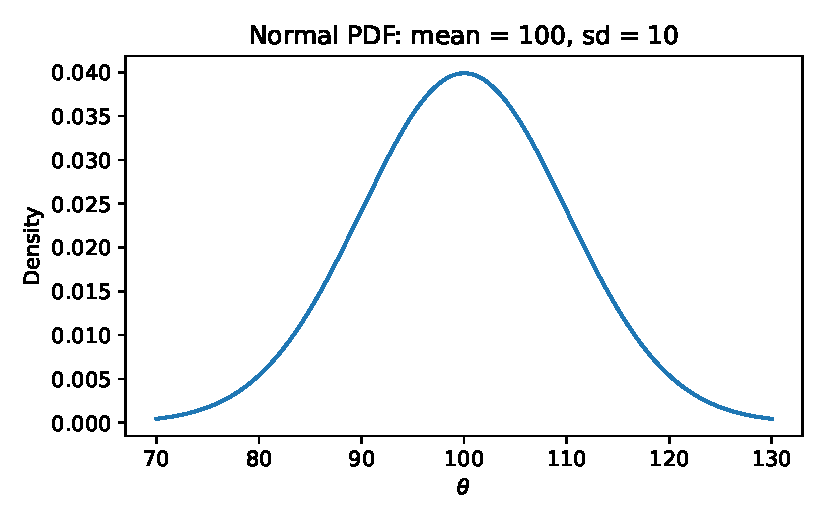
\includegraphics[keepaspectratio]{lectures/part2/5_bayes_parameter_estimation_files/figure-pdf/unnamed-chunk-1-1.pdf}}

\subsection{R}

\begin{Shaded}
\begin{Highlighting}[]
\NormalTok{mean }\OtherTok{\textless{}{-}} \DecValTok{100}
\NormalTok{sd   }\OtherTok{\textless{}{-}} \DecValTok{10}

\NormalTok{theta\_grid }\OtherTok{\textless{}{-}} \FunctionTok{seq}\NormalTok{(mean }\SpecialCharTok{{-}} \DecValTok{3}\SpecialCharTok{*}\NormalTok{sd, mean }\SpecialCharTok{+} \DecValTok{3}\SpecialCharTok{*}\NormalTok{sd, }\AttributeTok{length.out =} \DecValTok{200}\NormalTok{)}
\NormalTok{pdf\_values }\OtherTok{\textless{}{-}} \FunctionTok{dnorm}\NormalTok{(theta\_grid, }\AttributeTok{mean =}\NormalTok{ mean, }\AttributeTok{sd =}\NormalTok{ sd)}

\FunctionTok{plot}\NormalTok{(theta\_grid, pdf\_values, }\AttributeTok{type =} \StringTok{"l"}\NormalTok{,}
     \AttributeTok{xlab =} \FunctionTok{expression}\NormalTok{(theta),}
     \AttributeTok{ylab =} \StringTok{"Density"}\NormalTok{,}
     \AttributeTok{main =} \StringTok{"Normal PDF: mean = 100, sd = 10"}\NormalTok{)}
\end{Highlighting}
\end{Shaded}

\pandocbounded{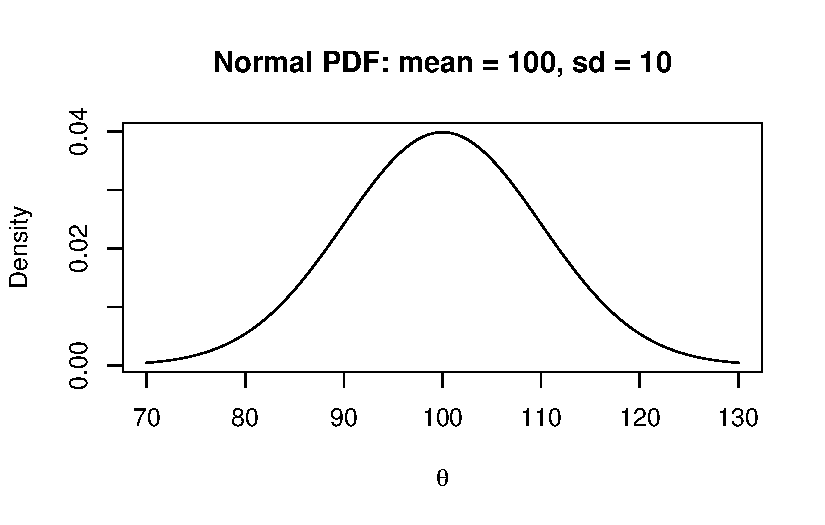
\includegraphics[keepaspectratio]{lectures/part2/5_bayes_parameter_estimation_files/figure-pdf/unnamed-chunk-2-3.pdf}}

\section{asdsss}\label{asdsss}

\part{Part III - Interval Estimation}

\part{Part IV --- Hypothesis Testing}

\part{Additional Material}

\chapter{Formula Sheet}\label{formula-sheet}

\section{Discrete distributions}\label{discrete-distributions}

\subsection{Bernoulli}\label{bern}

\textbf{Model.} \(X \sim \operatorname{Bernoulli}(p)\) with \(0<p<1\).\\
\textbf{Support.} \(x \in \{0,1\}\).\\
\textbf{PMF.} \[
\mathrm{Pr}(X=x) = p^{\,x}(1-p)^{1-x}, \quad x\in\{0,1\}.
\] \textbf{Mean/Var.}
\(\mathbb{E}[X]=p,\quad \operatorname{Var}(X)=p(1-p).\)

\subsection{Binomial}\label{binom}

\textbf{Model.} \(X \sim \operatorname{Bin}(n,p)\), \(n\in\mathbb{N}\),
\(0<p<1\).\\
\textbf{Support.} \(x=0,1,\ldots,n\).\\
\textbf{PMF.} \[
\mathrm{Pr}(X=x) = \binom{n}{x} p^x (1-p)^{n-x}.
\] \textbf{Mean/Var.}
\(\mathbb{E}[X]=np,\quad \operatorname{Var}(X)=np(1-p).\)

\subsection{Poisson}\label{pois}

\textbf{Model.} \(X \sim \operatorname{Po}(\lambda)\), \(\lambda>0\).\\
\textbf{Support.} \(x=0,1,2,\ldots\).\\
\textbf{PMF.} \[
\mathrm{Pr}(X=x)=\frac{\lambda^x e^{-\lambda}}{x!}.
\] \textbf{Mean/Var.}
\(\mathbb{E}[X]=\lambda,\quad \operatorname{Var}(X)=\lambda.\)

\section{Geometric}\label{geom}

\textbf{Model.} \(X \sim \operatorname{Geom}(p)\) (trials \textbf{until
first success}, counting the success), \(0<p<1\).\\
\textbf{Support.} \(x=1,2,\ldots\).\\
\textbf{PMF.} \[
\mathrm{Pr}(X=x)=p(1-p)^{x-1}.
\] \textbf{Mean/Var.}
\(\mathbb{E}[X]=\frac{1}{p},\quad \operatorname{Var}(X)=\frac{1-p}{p^2}.\)

\begin{tcolorbox}[enhanced jigsaw, left=2mm, titlerule=0mm, bottomrule=.15mm, colframe=quarto-callout-tip-color-frame, arc=.35mm, colback=white, breakable, title=\textcolor{quarto-callout-tip-color}{\faLightbulb}\hspace{0.5em}{Tip}, colbacktitle=quarto-callout-tip-color!10!white, opacitybacktitle=0.6, opacityback=0, toprule=.15mm, leftrule=.75mm, coltitle=black, toptitle=1mm, rightrule=.15mm, bottomtitle=1mm]

\textbf{Alternative convention.} Some texts start at \(x=0\) (failures
before the first success). Adjust mean/variance accordingly.

\end{tcolorbox}

\subsection{Negative Binomial}\label{negbin}

\textbf{Model.} \(X \sim \operatorname{NegBin}(r,p)\): number of trials
to achieve the \(r\)-th success (counts the successes), \(r>0\) (often
integer), \(0<p<1\).\\
\textbf{Support.} \(x=r,r+1,\ldots\).\\
\textbf{PMF.} \[
\mathrm{Pr}(X=x) = \binom{x-1}{r-1} p^{\,r} (1-p)^{x-r}.
\] \textbf{Mean/Var.}
\(\mathbb{E}[X]=\frac{r}{p},\quad \operatorname{Var}(X)=\frac{r(1-p)}{p^2}.\)

\begin{tcolorbox}[enhanced jigsaw, left=2mm, titlerule=0mm, bottomrule=.15mm, colframe=quarto-callout-warning-color-frame, arc=.35mm, colback=white, breakable, title=\textcolor{quarto-callout-warning-color}{\faExclamationTriangle}\hspace{0.5em}{Warning}, colbacktitle=quarto-callout-warning-color!10!white, opacitybacktitle=0.6, opacityback=0, toprule=.15mm, leftrule=.75mm, coltitle=black, toptitle=1mm, rightrule=.15mm, bottomtitle=1mm]

\textbf{Parameterisation alert.} Another common version counts
\textbf{failures} before the \(r\)-th success (\(x=0,1,\dots\)) with
different mean/variance. Always check which one is used.

\end{tcolorbox}

\section{Continuous distributions}\label{continuous-distributions}

\subsection{Uniform (continuous)}\label{unif}

\textbf{Model.} \(X \sim \operatorname{Unif}(a,b)\), \(a<b\).\\
\textbf{Support.} \(a<x<b\).\\
\textbf{PDF.} \[
f_X(x;a,b)=\frac{1}{b-a}.
\] \textbf{Mean/Var.}
\(\mathbb{E}[X]=\frac{a+b}{2},\quad \operatorname{Var}(X)=\frac{(b-a)^2}{12}.\)

\section{Exponential}\label{exp}

\textbf{Model.} \(X \sim \operatorname{Exp}(\lambda)\) with
\textbf{rate} \(\lambda>0\).\\
\textbf{Support.} \(x>0\).\\
\textbf{PDF.} \[
f_X(x;\lambda)=\lambda e^{-\lambda x}.
\] \textbf{Mean/Var.}
\(\mathbb{E}[X]=\frac{1}{\lambda},\quad \operatorname{Var}(X)=\frac{1}{\lambda^2}.\)

\subsection{Gamma}\label{gamma}

\textbf{Model.} \(X \sim \operatorname{Gamma}(a,b)\) with \textbf{shape}
\(a>0\) and \textbf{rate} \(b>0\).\\
\textbf{Support.} \(x>0\).\\
\textbf{PDF.} \[
f_X(x;a,b)=\frac{b^a}{\Gamma(a)} x^{a-1} e^{-bx}.
\] \textbf{Mean/Var.}
\(\mathbb{E}[X]=\frac{a}{b},\quad \operatorname{Var}(X)=\frac{a}{b^2}.\)

\begin{tcolorbox}[enhanced jigsaw, left=2mm, titlerule=0mm, bottomrule=.15mm, colframe=quarto-callout-tip-color-frame, arc=.35mm, colback=white, breakable, title=\textcolor{quarto-callout-tip-color}{\faLightbulb}\hspace{0.5em}{Tip}, colbacktitle=quarto-callout-tip-color!10!white, opacitybacktitle=0.6, opacityback=0, toprule=.15mm, leftrule=.75mm, coltitle=black, toptitle=1mm, rightrule=.15mm, bottomtitle=1mm]

Many sources use \textbf{scale} \(\beta=1/b\): then
\(f(x)=\frac{1}{\Gamma(a)\beta^a}x^{a-1}e^{-x/\beta}\) and
\(\mathbb{E}[X]=a\beta\).

\end{tcolorbox}

\subsection{Normal}\label{normal}

\textbf{Model.} \(X \sim \mathcal{N}(\mu,\sigma^2)\) with
\(\sigma>0\).\\
\textbf{Support.} \(x\in\mathbb{R}\).\\
\textbf{PDF.} \[
f_X(x;\mu,\sigma^2)=\frac{1}{\sqrt{2\pi \sigma^2}}
\exp\!\left(-\frac{(x-\mu)^2}{2\sigma^2}\right).
\] \textbf{Mean/Var.}
\(\mathbb{E}[X]=\mu,\quad \operatorname{Var}(X)=\sigma^2.\)

\subsection{Lognormal}\label{lognormal}

\textbf{Model.} \(X \sim \operatorname{LogNormal}(\mu,\sigma^2)\)
meaning \(\ln X \sim \mathcal{N}(\mu,\sigma^2)\).\\
\textbf{Support.} \(x>0\).\\
\textbf{PDF.} \[
f_X(x;\mu,\sigma^2)=\frac{1}{x\sqrt{2\pi\sigma^2}}
\exp\!\left(-\frac{(\ln x-\mu)^2}{2\sigma^2}\right).
\] \textbf{Mean/Var.}
\(\mathbb{E}[X]=e^{\mu+\sigma^2/2},\quad \operatorname{Var}(X)=\big(e^{\sigma^2}-1\big)e^{2\mu+\sigma^2}.\)

\subsection{Chi-squared}\label{chisq}

\textbf{Model.} \(X \sim \chi^2_\nu\) with \(\nu>0\) degrees of
freedom.\\
\textbf{Support.} \(x>0\).\\
\textbf{PDF.} \[
f_X(x;\nu)=\frac{1}{2^{\nu/2}\Gamma(\nu/2)}x^{\nu/2-1}e^{-x/2}.
\] \textbf{Mean/Var.}
\(\mathbb{E}[X]=\nu,\quad \operatorname{Var}(X)=2\nu.\)

\begin{tcolorbox}[enhanced jigsaw, left=2mm, titlerule=0mm, bottomrule=.15mm, colframe=quarto-callout-note-color-frame, arc=.35mm, colback=white, breakable, title=\textcolor{quarto-callout-note-color}{\faInfo}\hspace{0.5em}{Note}, colbacktitle=quarto-callout-note-color!10!white, opacitybacktitle=0.6, opacityback=0, toprule=.15mm, leftrule=.75mm, coltitle=black, toptitle=1mm, rightrule=.15mm, bottomtitle=1mm]

\(\chi^2_\nu\) is a special case of Gamma with \(a=\nu/2\), \(b=1/2\).

\end{tcolorbox}

\subsection{\texorpdfstring{Student-\(t\)}{Student-t}}\label{t}

\textbf{Model.} \(X \sim t_\nu\) with \(\nu>0\) degrees of freedom.\\
\textbf{Support.} \(x\in\mathbb{R}\).\\
\textbf{PDF.} \[
f_X(x;\nu)=\frac{\Gamma\!\left(\frac{\nu+1}{2}\right)}{\sqrt{\nu\pi}\,\Gamma\!\left(\frac{\nu}{2}\right)}
\left(1+\frac{x^2}{\nu}\right)^{-(\nu+1)/2}.
\] \textbf{Mean/Var.} \(\mathbb{E}[X]=0\) for \(\nu>1\); undefined for
\(\nu\le 1\).\\
\(\operatorname{Var}(X)=\frac{\nu}{\nu-2}\) for \(\nu>2\); infinite for
\(1<\nu\le 2\); undefined for \(\nu\le 1\).

\subsection{\texorpdfstring{\(F\)
distribution}{F distribution}}\label{f}

\textbf{Model.} \(X \sim F_{d_1,d_2}\) with \(d_1,d_2>0\) degrees of
freedom.\\
\textbf{Support.} \(x>0\).\\
\textbf{PDF.} \[
f_X(x;d_1,d_2)=\frac{\Gamma\!\left(\frac{d_1+d_2}{2}\right)}{\Gamma\!\left(\frac{d_1}{2}\right)\Gamma\!\left(\frac{d_2}{2}\right)}
\left(\frac{d_1}{d_2}\right)^{d_1/2}\frac{x^{d_1/2-1}}{\left(1+\frac{d_1}{d_2}x\right)^{(d_1+d_2)/2}}.
\] \textbf{Mean/Var.} \(\mathbb{E}[X]=\frac{d_2}{d_2-2}\) for
\(d_2>2\).\\
\(\operatorname{Var}(X)=\frac{2d_2^2(d_1+d_2-2)}{d_1(d_2-2)^2(d_2-4)}\)
for \(d_2>4\).

\section{Beta}\label{beta}

\textbf{Model.} \(X \sim \operatorname{Beta}(a,b)\), \(a>0, b>0\).\\
\textbf{Support.} \(0<x<1\).\\
\textbf{PDF.} \[
f_X(x;a,b)=\frac{\Gamma(a+b)}{\Gamma(a)\Gamma(b)}\,x^{a-1}(1-x)^{b-1}.
\] \textbf{Mean/Var.}
\(\mathbb{E}[X]=\frac{a}{a+b},\quad \operatorname{Var}(X)=\frac{ab}{(a+b)^2(a+b+1)}.\)

\subsection{Multivariate Normal}\label{mvnorm}

\textbf{Model.}
\(\mathbf{X} \sim \mathcal{N}_p(\boldsymbol{\mu},\Sigma)\) with
\(\Sigma\) positive definite.\\
\textbf{Support.} \(\mathbf{x}\in\mathbb{R}^p\).\\
\textbf{PDF.} \[
f_{\mathbf{X}}(\mathbf{x};\boldsymbol{\mu},\Sigma)=\frac{1}{(2\pi)^{p/2}(\det\Sigma)^{1/2}}
\exp\!\left(-\tfrac{1}{2}(\mathbf{x}-\boldsymbol{\mu})^\top \Sigma^{-1}(\mathbf{x}-\boldsymbol{\mu})\right).
\] \textbf{Mean/Cov.}
\(\mathbb{E}[\mathbf{X}]=\boldsymbol{\mu},\quad \operatorname{Var}(\mathbf{X})=\Sigma.\)

\begin{center}\rule{0.5\linewidth}{0.5pt}\end{center}

\section{Integral reminder}\label{integral-reminder}

The Gamma function: \[
\Gamma(a)=\int_0^\infty x^{a-1}e^{-x}\,dx, \qquad a>0.
\]

\begin{tcolorbox}[enhanced jigsaw, left=2mm, titlerule=0mm, bottomrule=.15mm, colframe=quarto-callout-important-color-frame, arc=.35mm, colback=white, breakable, title=\textcolor{quarto-callout-important-color}{\faExclamation}\hspace{0.5em}{Important}, colbacktitle=quarto-callout-important-color!10!white, opacitybacktitle=0.6, opacityback=0, toprule=.15mm, leftrule=.75mm, coltitle=black, toptitle=1mm, rightrule=.15mm, bottomtitle=1mm]

\textbf{Common pitfalls.} - \textbf{Rate vs scale} for
Exponential/Gamma: check whether the parameter is \(\lambda\) (rate) or
\(\beta\) (scale). - \textbf{Geometric/Negative Binomial} supports vary
by convention (counting failures vs trials). Always verify support and
mean/variance before using formulas. - In likelihood work, write
\(f_X(x;\theta)\) (semicolon) to emphasise \textbf{data vs parameters}.

\end{tcolorbox}

\chapter{Revision Sheet}\label{revision-sheet}




\end{document}
